% Options for packages loaded elsewhere
\PassOptionsToPackage{unicode}{hyperref}
\PassOptionsToPackage{hyphens}{url}
\PassOptionsToPackage{dvipsnames,svgnames,x11names}{xcolor}
%
\documentclass[
  12pt,
  a4paper,
]{article}
\usepackage{amsmath,amssymb}
\usepackage{setspace}
\usepackage{iftex}
\ifPDFTeX
  \usepackage[T1]{fontenc}
  \usepackage[utf8]{inputenc}
  \usepackage{textcomp} % provide euro and other symbols
\else % if luatex or xetex
  \usepackage{unicode-math} % this also loads fontspec
  \defaultfontfeatures{Scale=MatchLowercase}
  \defaultfontfeatures[\rmfamily]{Ligatures=TeX,Scale=1}
\fi
\usepackage{lmodern}
\ifPDFTeX\else
  % xetex/luatex font selection
  \setmainfont[]{Tinos}
\fi
% Use upquote if available, for straight quotes in verbatim environments
\IfFileExists{upquote.sty}{\usepackage{upquote}}{}
\IfFileExists{microtype.sty}{% use microtype if available
  \usepackage[]{microtype}
  \UseMicrotypeSet[protrusion]{basicmath} % disable protrusion for tt fonts
}{}
\makeatletter
\@ifundefined{KOMAClassName}{% if non-KOMA class
  \IfFileExists{parskip.sty}{%
    \usepackage{parskip}
  }{% else
    \setlength{\parindent}{0pt}
    \setlength{\parskip}{6pt plus 2pt minus 1pt}}
}{% if KOMA class
  \KOMAoptions{parskip=half}}
\makeatother
\usepackage{xcolor}
\usepackage[margin=2.1cm]{geometry}
\usepackage{color}
\usepackage{fancyvrb}
\newcommand{\VerbBar}{|}
\newcommand{\VERB}{\Verb[commandchars=\\\{\}]}
\DefineVerbatimEnvironment{Highlighting}{Verbatim}{commandchars=\\\{\}}
% Add ',fontsize=\small' for more characters per line
\newenvironment{Shaded}{}{}
\newcommand{\AlertTok}[1]{\textcolor[rgb]{1.00,0.00,0.00}{\textbf{#1}}}
\newcommand{\AnnotationTok}[1]{\textcolor[rgb]{0.38,0.63,0.69}{\textbf{\textit{#1}}}}
\newcommand{\AttributeTok}[1]{\textcolor[rgb]{0.49,0.56,0.16}{#1}}
\newcommand{\BaseNTok}[1]{\textcolor[rgb]{0.25,0.63,0.44}{#1}}
\newcommand{\BuiltInTok}[1]{\textcolor[rgb]{0.00,0.50,0.00}{#1}}
\newcommand{\CharTok}[1]{\textcolor[rgb]{0.25,0.44,0.63}{#1}}
\newcommand{\CommentTok}[1]{\textcolor[rgb]{0.38,0.63,0.69}{\textit{#1}}}
\newcommand{\CommentVarTok}[1]{\textcolor[rgb]{0.38,0.63,0.69}{\textbf{\textit{#1}}}}
\newcommand{\ConstantTok}[1]{\textcolor[rgb]{0.53,0.00,0.00}{#1}}
\newcommand{\ControlFlowTok}[1]{\textcolor[rgb]{0.00,0.44,0.13}{\textbf{#1}}}
\newcommand{\DataTypeTok}[1]{\textcolor[rgb]{0.56,0.13,0.00}{#1}}
\newcommand{\DecValTok}[1]{\textcolor[rgb]{0.25,0.63,0.44}{#1}}
\newcommand{\DocumentationTok}[1]{\textcolor[rgb]{0.73,0.13,0.13}{\textit{#1}}}
\newcommand{\ErrorTok}[1]{\textcolor[rgb]{1.00,0.00,0.00}{\textbf{#1}}}
\newcommand{\ExtensionTok}[1]{#1}
\newcommand{\FloatTok}[1]{\textcolor[rgb]{0.25,0.63,0.44}{#1}}
\newcommand{\FunctionTok}[1]{\textcolor[rgb]{0.02,0.16,0.49}{#1}}
\newcommand{\ImportTok}[1]{\textcolor[rgb]{0.00,0.50,0.00}{\textbf{#1}}}
\newcommand{\InformationTok}[1]{\textcolor[rgb]{0.38,0.63,0.69}{\textbf{\textit{#1}}}}
\newcommand{\KeywordTok}[1]{\textcolor[rgb]{0.00,0.44,0.13}{\textbf{#1}}}
\newcommand{\NormalTok}[1]{#1}
\newcommand{\OperatorTok}[1]{\textcolor[rgb]{0.40,0.40,0.40}{#1}}
\newcommand{\OtherTok}[1]{\textcolor[rgb]{0.00,0.44,0.13}{#1}}
\newcommand{\PreprocessorTok}[1]{\textcolor[rgb]{0.74,0.48,0.00}{#1}}
\newcommand{\RegionMarkerTok}[1]{#1}
\newcommand{\SpecialCharTok}[1]{\textcolor[rgb]{0.25,0.44,0.63}{#1}}
\newcommand{\SpecialStringTok}[1]{\textcolor[rgb]{0.73,0.40,0.53}{#1}}
\newcommand{\StringTok}[1]{\textcolor[rgb]{0.25,0.44,0.63}{#1}}
\newcommand{\VariableTok}[1]{\textcolor[rgb]{0.10,0.09,0.49}{#1}}
\newcommand{\VerbatimStringTok}[1]{\textcolor[rgb]{0.25,0.44,0.63}{#1}}
\newcommand{\WarningTok}[1]{\textcolor[rgb]{0.38,0.63,0.69}{\textbf{\textit{#1}}}}
\usepackage{longtable,booktabs,array}
\usepackage{calc} % for calculating minipage widths
% Correct order of tables after \paragraph or \subparagraph
\usepackage{etoolbox}
\makeatletter
\patchcmd\longtable{\par}{\if@noskipsec\mbox{}\fi\par}{}{}
\makeatother
% Allow footnotes in longtable head/foot
\IfFileExists{footnotehyper.sty}{\usepackage{footnotehyper}}{\usepackage{footnote}}
\makesavenoteenv{longtable}
\usepackage{graphicx}
\makeatletter
\def\maxwidth{\ifdim\Gin@nat@width>\linewidth\linewidth\else\Gin@nat@width\fi}
\def\maxheight{\ifdim\Gin@nat@height>\textheight\textheight\else\Gin@nat@height\fi}
\makeatother
% Scale images if necessary, so that they will not overflow the page
% margins by default, and it is still possible to overwrite the defaults
% using explicit options in \includegraphics[width, height, ...]{}
\setkeys{Gin}{width=\maxwidth,height=\maxheight,keepaspectratio}
% Set default figure placement to htbp
\makeatletter
\def\fps@figure{htbp}
\makeatother
\setlength{\emergencystretch}{3em} % prevent overfull lines
\providecommand{\tightlist}{%
  \setlength{\itemsep}{0pt}\setlength{\parskip}{0pt}}
\setcounter{secnumdepth}{-\maxdimen} % remove section numbering
\ifLuaTeX
\usepackage[bidi=basic]{babel}
\else
\usepackage[bidi=default]{babel}
\fi
\babelprovide[main,import]{vietnamese}
\ifPDFTeX
\else
\babelfont{rm}[]{Tinos}
\fi
% get rid of language-specific shorthands (see #6817):
\let\LanguageShortHands\languageshorthands
\def\languageshorthands#1{}
\ifLuaTeX
  \usepackage{selnolig}  % disable illegal ligatures
\fi
\usepackage{bookmark}
\IfFileExists{xurl.sty}{\usepackage{xurl}}{} % add URL line breaks if available
\urlstyle{same}
\hypersetup{
  pdftitle={Động học, động lực học và PID robot vi sai},
  pdfauthor={Nguyễn Hoàng Anh \textbar{} Nhóm Industrial AMR Robot},
  pdflang={vi-VN},
  colorlinks=true,
  linkcolor={Maroon},
  filecolor={Maroon},
  citecolor={Blue},
  urlcolor={Blue},
  pdfcreator={LaTeX via pandoc}}

\title{Động học, động lực học và PID robot vi sai}
\usepackage{etoolbox}
\makeatletter
\providecommand{\subtitle}[1]{% add subtitle to \maketitle
  \apptocmd{\@title}{\par {\large #1 \par}}{}{}
}
\makeatother
\subtitle{Factory Delivery AMR --- Báo cáo kỹ thuật kèm đồ thị và mã
MATLAB}
\author{Nguyễn Hoàng Anh \textbar{} Nhóm Industrial AMR Robot}
\date{10/11/2026 --- Bản cập nhật phục vụ GitHub nhóm}

\begin{document}
\maketitle

{
\hypersetup{linkcolor=}
\setcounter{tocdepth}{3}
\tableofcontents
}
\setstretch{1.15}
\begin{quote}
\textbf{Phạm vi:} báo cáo mô hình số và lý thuyết điều khiển; chưa phải
báo cáo thử nghiệm Gazebo/robot thật.
\end{quote}

\section{1. Mục tiêu, phạm vi và quy ước dữ
liệu}\label{mux1ee5c-tiuxeau-phux1ea1m-vi-vuxe0-quy-ux1b0ux1edbc-dux1eef-liux1ec7u}

Tài liệu phục vụ nhiệm vụ được phân công: tổng hợp cơ sở toán học của
robot di động truyền động vi sai, đưa ra mô hình động lực học ở mức đủ
xây dựng bộ điều khiển tốc độ bánh xe, giải thích PI/PID, và xác định
cách kiểm tra bằng mô phỏng.

Nội dung được xây dựng cho bài toán Factory Delivery AMR: robot nhận
khay từ kho A, giao đến B → C → D; tải hữu ích \textbf{20 kg}, hành lang
\textbf{1,2 m}, vận tốc yêu cầu \textbf{≥ 1,2 m/s}, sai số dừng
\textbf{\textless{} 30 mm} theo tiêu chí cần chốt và thời gian hoạt động
\textbf{≥ 4 giờ}. Các con số này là yêu cầu ban đầu từ khách hàng, không
phải kết quả robot đã đạt.

\textbf{Tình trạng liên kết mã nguồn:} repository nhóm:
\href{https://github.com/HoangAnh301194/Industrial_AMR_Robot}{HoangAnh301194/Industrial\_AMR\_Robot}.
Chưa đối chiếu được nội dung riêng của repository với các giá trị giả
định trong tài liệu này. Trước khi nhập cấu hình vào URDF / Gazebo, nhóm
phải lấy \texttt{wheel\_radius}, \texttt{wheel\_separation}, khối lượng
và quán tính trực tiếp từ model hiện hành.

\begin{longtable}[]{@{}
  >{\raggedright\arraybackslash}p{(\columnwidth - 6\tabcolsep) * \real{0.2500}}
  >{\raggedright\arraybackslash}p{(\columnwidth - 6\tabcolsep) * \real{0.2500}}
  >{\raggedleft\arraybackslash}p{(\columnwidth - 6\tabcolsep) * \real{0.2500}}
  >{\raggedright\arraybackslash}p{(\columnwidth - 6\tabcolsep) * \real{0.2500}}@{}}
\toprule\noalign{}
\begin{minipage}[b]{\linewidth}\raggedright
Nhóm dữ liệu
\end{minipage} & \begin{minipage}[b]{\linewidth}\raggedright
Đại lượng
\end{minipage} & \begin{minipage}[b]{\linewidth}\raggedleft
Giá trị
\end{minipage} & \begin{minipage}[b]{\linewidth}\raggedright
Trạng thái
\end{minipage} \\
\midrule\noalign{}
\endhead
\bottomrule\noalign{}
\endlastfoot
Khách hàng & Tải hữu ích & 20 kg & Đầu vào đã nêu \\
Khách hàng & Hành lang & 1,20 m & Đầu vào đã nêu \\
Khách hàng & Vận tốc tối thiểu yêu cầu & 1,20 m/s & Cần chốt điều kiện
đo \\
Khách hàng & Sai số dừng & \textless{} 30 mm & Cần chốt phép đo nghiệm
thu \\
Khách hàng & Thời gian hoạt động & ≥ 4 giờ & Cần chốt duty cycle \\
Minh họa & Kích thước bao hình & 0,70 × 0,55 m & Đề xuất sơ bộ \\
Minh họa & Khối lượng thân + thiết bị & 55 kg & Giả định, chưa cân đo \\
Minh họa & Tổng khối lượng khi tải & 75 kg & 55 + 20 kg \\
Minh họa & Bán kính bánh chủ động, \(r\) & 0,08 m & Giả định bánh Ø160
mm \\
Minh họa & Khoảng cách tâm bánh, \(b\) & 0,45 m & \textbf{Giả định}, cần
đọc URDF \\
Minh họa & Gia tốc thiết kế, \(a\) & 0,80 m/s² & Giả định để tính
chọn \\
Minh họa & Hệ số cản lăn, \(c_{rr}\) & 0,025 & Giả định; phụ thuộc
sàn/bánh \\
Minh họa & Hệ số dự phòng lực, \(k_s\) & 1,5 & Giả định thiết kế \\
\end{longtable}

Tất cả phương trình sử dụng hệ SI. Trục \(x\) của robot hướng về phía
trước, \(y\) sang trái và \(z\) hướng lên; \(\theta\) dương theo chiều
ngược kim đồng hồ. Hai bánh chủ động được ký hiệu \textbf{trái (L)} và
\textbf{phải (R)}; bánh caster chỉ đỡ tải và không tạo lực chủ động lý
tưởng. Robot có thể có 4 bánh \emph{vật lý} (2 chủ động + 2 caster),
nhưng mô hình động học vi sai chỉ cần hai bánh chủ động.

\begin{figure}
\centering
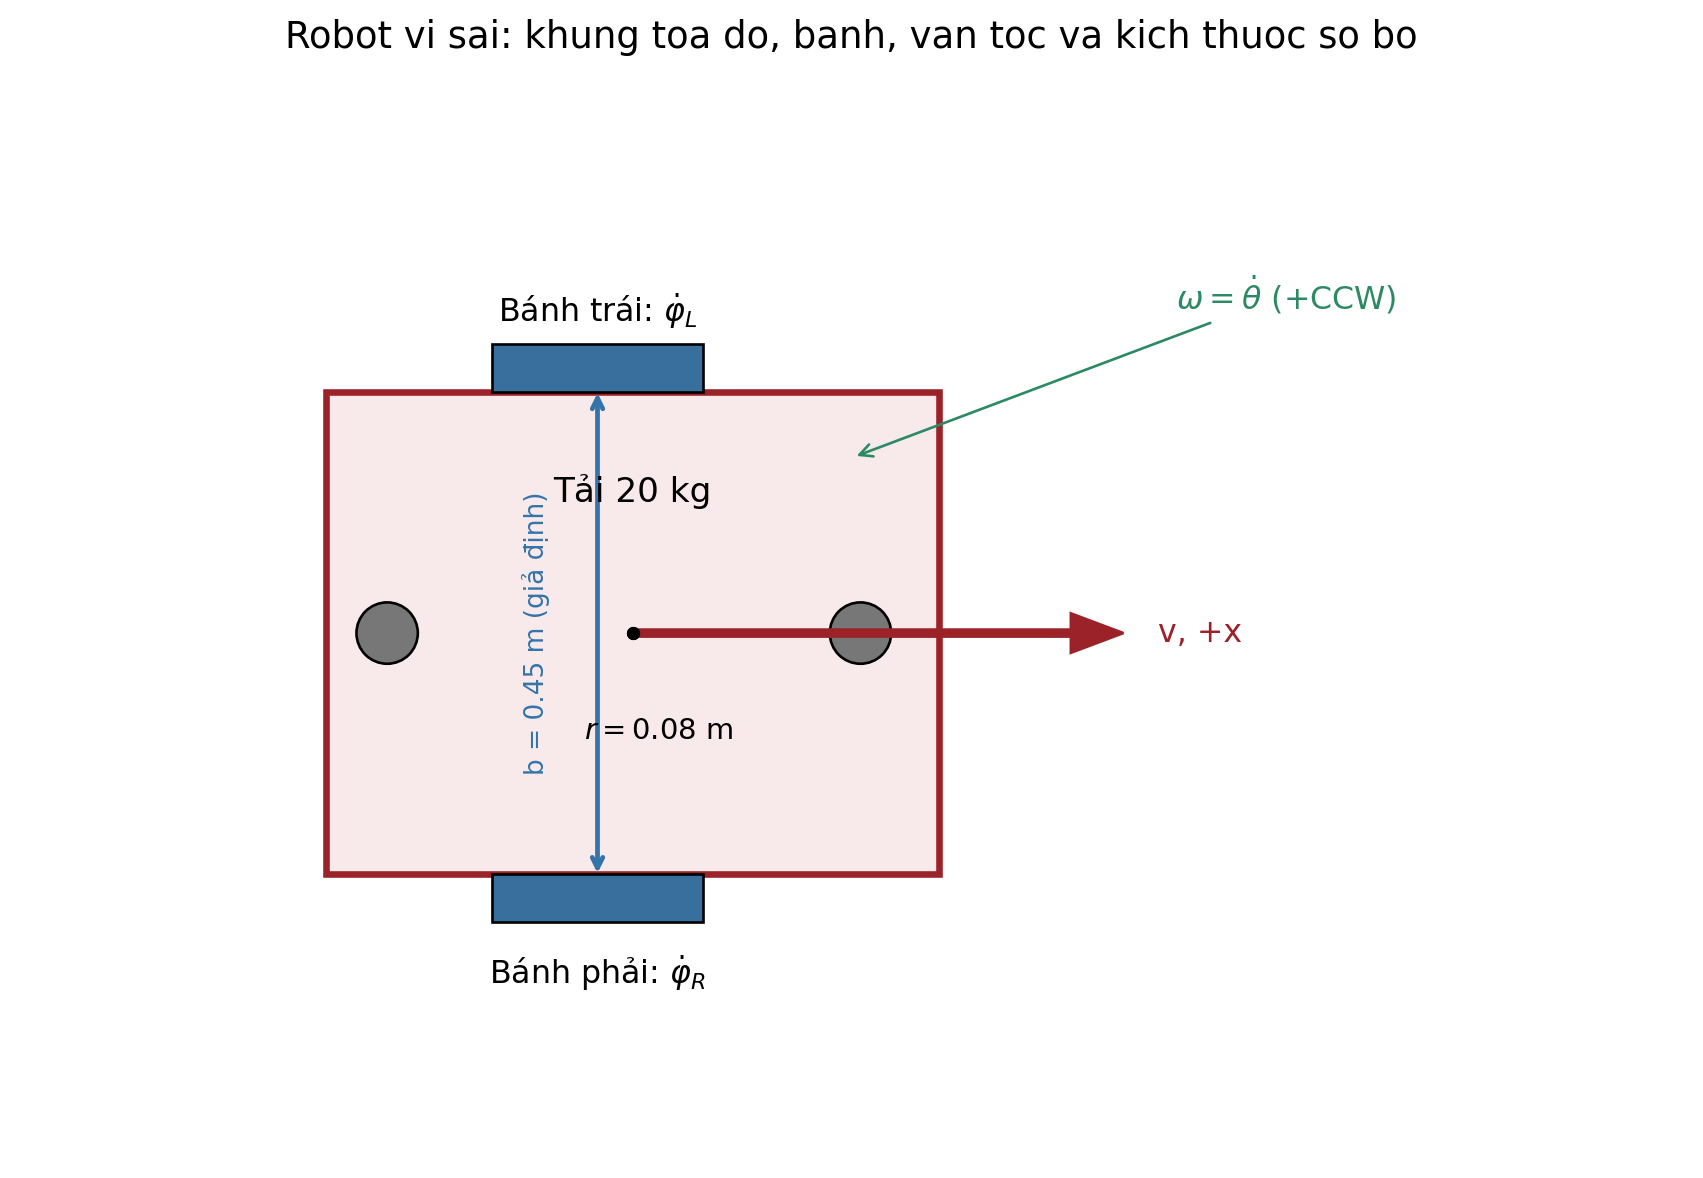
\includegraphics{assets/diff_drive_geometry.png}
\caption{Hình 1. Hình học robot vi sai và quy ước tọa độ.}
\end{figure}

\section{2. Động học robot vi sai hai
bánh}\label{ux111ux1ed9ng-hux1ecdc-robot-vi-sai-hai-buxe1nh}

\subsection{2.1. Các giả thiết mô
hình}\label{cuxe1c-giux1ea3-thiux1ebft-muxf4-huxecnh}

Nền phẳng, tiếp xúc bánh--sàn không trượt thuần; bánh trái và phải có
cùng bán kính hiệu dụng \(r\); tâm robot là trung điểm hai bánh chủ
động; tốc độ của bánh có thể đo bằng encoder. Chuyển động ngang tức thời
trong hệ trục robot được coi bằng 0 (ràng buộc không trượt ngang). Khi
có trượt bánh, sàn dốc, tải lệch hoặc bánh caster bị rung, mô hình này
chỉ là xấp xỉ.

\subsection{2.2. Động học
thuận}\label{ux111ux1ed9ng-hux1ecdc-thuux1eadn}

Ký hiệu \(\dot{\varphi}_R,\dot{\varphi}_L\) là vận tốc góc bánh
phải/trái (rad/s), \(v\) là vận tốc tiến và \(\omega=\dot{\theta}\) là
vận tốc quay thân (rad/s):

\[
v=\frac{r}{2}(\dot{\varphi}_R+\dot{\varphi}_L),\qquad
\omega=\frac{r}{b}(\dot{\varphi}_R-\dot{\varphi}_L).
\]

Dạng ma trận, với thứ tự hai bánh \([R,L]^T\):

\[
\begin{bmatrix}v\\\omega\end{bmatrix}=
\begin{bmatrix}r/2&r/2\\r/b&-r/b\end{bmatrix}
\begin{bmatrix}\dot{\varphi}_R\\\dot{\varphi}_L\end{bmatrix}.
\]

Chuyển từ vận tốc trong hệ robot sang đạo hàm tư thế trong hệ bản đồ:

\[
\dot{x}=v\cos\theta,\qquad
\dot{y}=v\sin\theta,\qquad
\dot{\theta}=\omega.
\]

\textbf{Các trường hợp quan trọng:} \(\dot{\varphi}_R=\dot{\varphi}_L\)
→ đi thẳng; \(\dot{\varphi}_R=-\dot{\varphi}_L\) → quay gần như tại tâm;
hai tốc độ khác nhau → chuyển động cong. Nếu \(\omega\neq0\), bán kính
cong quỹ đạo của tâm là \(R_c=v/\omega\).

\subsection{2.3. Động học
nghịch}\label{ux111ux1ed9ng-hux1ecdc-nghux1ecbch}

Cho lệnh tốc độ thân từ điều hướng \(v^*,\omega^*\), tính tốc độ đặt của
hai bánh:

\[
\boxed{\dot{\varphi}_R^*=\frac{v^*+\tfrac b2\omega^*}{r}},\qquad
\boxed{\dot{\varphi}_L^*=\frac{v^*-\tfrac b2\omega^*}{r}}.
\]

Ví dụ với \(r=0,08\) m, \(b=0,45\) m và lệnh đi thẳng \(v^*=1,20\) m/s,
\(\omega^*=0\): cả hai bánh cần đạt \(15\) rad/s, tương đương
\(15\times60/(2\pi)=143,24\) vòng/phút. Khi \(v^*=0,60\) m/s và
\(\omega^*=0,50\) rad/s, ta có \(\dot{\varphi}_R^*=8,906\) rad/s và
\(\dot{\varphi}_L^*=6,094\) rad/s, cho bán kính cong lý thuyết \(1,20\)
m. Nếu tỷ số truyền là \(i=10\), tốc độ motor khi xe chạy thẳng 1,2 m/s
xấp xỉ \(1432,4\) vòng/phút (bỏ qua trượt bánh).

\subsection{2.4. Odometry và phép biến đổi
TF}\label{odometry-vuxe0-phuxe9p-biux1ebfn-ux111ux1ed5i-tf}

Encoder cho biết độ thay đổi góc bánh
\(\Delta\varphi_R,\Delta\varphi_L\). Từ đó:

\[
\Delta s=\frac r2(\Delta\varphi_R+\Delta\varphi_L),\qquad
\Delta\theta=\frac rb(\Delta\varphi_R-\Delta\varphi_L).
\]

Cập nhật tư thế bằng góc giữa bước:

\[
x_{k+1}=x_k+\Delta s\cos(\theta_k+\Delta\theta/2),\qquad
 y_{k+1}=y_k+\Delta s\sin(\theta_k+\Delta\theta/2),\qquad
\theta_{k+1}=\theta_k+\Delta\theta.
\]

Chuỗi TF dự kiến được chia theo cây như sau:

\begin{Shaded}
\begin{Highlighting}[]
\NormalTok{map {-}\textgreater{} odom {-}\textgreater{} base\_link}
\NormalTok{base\_link {-}\textgreater{} laser\_link}
\NormalTok{base\_link {-}\textgreater{} imu\_link}
\NormalTok{base\_link {-}\textgreater{} wheel\_left\_link}
\NormalTok{base\_link {-}\textgreater{} wheel\_right\_link}
\end{Highlighting}
\end{Shaded}

\texttt{map→odom} thường do hệ định vị (SLAM/AMCL) phát;
\texttt{odom→base\_link} chỉ do \textbf{một} nguồn odometry/EKF phát.
Không để plugin Gazebo và EKF cùng phát một transform. Khi sai bán kính
bánh hoặc khoảng cách hai bánh trong URDF, odometry sẽ sai tỷ lệ quãng
đường hoặc góc quay.

\section{3. Động lực học robot vi
sai}\label{ux111ux1ed9ng-lux1ef1c-hux1ecdc-robot-vi-sai}

\subsection{3.1. Cân bằng lực theo phương chuyển
động}\label{cuxe2n-bux1eb1ng-lux1ef1c-theo-phux1b0ux1a1ng-chuyux1ec3n-ux111ux1ed9ng}

Khác động học (mô tả cách di chuyển), động lực học xét lực, mô-men, khối
lượng, gia tốc, ma sát và công suất. Trong mô hình phẳng đơn giản:

\[
m\dot{v}=\frac{\tau_{w,R}+\tau_{w,L}}{r}-F_{rr}-F_d-F_g,
\]

với \(\tau_{w,R},\tau_{w,L}\) là mô-men \textbf{tại trục bánh chủ động}.
Nếu mô-men được tính tại trục motor (\(\tau_m\)), cần quy đổi qua hộp
số: \(\tau_w=\eta_g i\tau_m\) (với \(i\) là tỷ số truyền và \(\eta_g\)
là hiệu suất). Như vậy lực kéo ở bánh là \((\tau_{w,R}+\tau_{w,L})/r\).
Cần nhất quán định nghĩa khi viết code và chọn động cơ.
\(F_{rr}\approx c_{rr}mg\) là lực cản lăn trên sàn ngang; \(F_d\) gồm
cản môi trường và tải phụ; \(F_g=mg\sin\alpha\) là thành phần trọng lực
khi sàn dốc góc \(\alpha\).

Theo chuyển động quay thân quanh trục \(z\):

\[
I_z\dot{\omega}=\frac{b}{2r}\big(\tau_{w,R}-\tau_{w,L}\big)-M_{\rm res},
\]

trong đó \(\tau_{w,R},\tau_{w,L}\) là mô-men bánh thực tế,
\(M_{\rm res}\) là mô-men cản quay. Công thức là xấp xỉ cho robot cứng,
không xét đầy đủ chuyển tải, rung caster và biến dạng bánh. Mỗi bánh
phải thỏa giới hạn bám đường; mô-men lớn không có nghĩa có thể truyền
hết lực xuống sàn.

\subsection{3.2. Mô hình quán tính ghép hai
bánh}\label{muxf4-huxecnh-quuxe1n-tuxednh-ghuxe9p-hai-buxe1nh}

Với \(\dot{\varphi}=[\dot{\varphi}_R,\dot{\varphi}_L]^T\), khối lượng
tổng \(m\), mô-men quán tính quay thân \(I_z\), quán tính quay mỗi bánh
\(J_w\) và bỏ qua trượt bánh:

\[
T=\frac12 mv^2+\frac12 I_z\omega^2+
\frac12J_w(\dot{\varphi}_R^2+\dot{\varphi}_L^2).
\]

Suy ra ma trận quán tính quy đổi đến trục bánh:

\[
\mathbf M_w =
\begin{bmatrix}
\frac{mr^2}{4}+\frac{I_zr^2}{b^2}+J_w &\frac{mr^2}{4}-\frac{I_zr^2}{b^2}\\
\frac{mr^2}{4}-\frac{I_zr^2}{b^2}&\frac{mr^2}{4}+\frac{I_zr^2}{b^2}+J_w
\end{bmatrix}.
\]

Phương trình rút gọn:

\[
\mathbf M_w\ddot{\boldsymbol\varphi}
=\begin{bmatrix}\tau_{w,R}\\\tau_{w,L}\end{bmatrix}
-\mathbf B_w\dot{\boldsymbol\varphi}
-\boldsymbol\tau_{\rm roll}.
\]

Quán tính \(I_z\) có thể \textbf{ước lượng sơ bộ} bằng hình hộp đồng
nhất \(I_z\approx m(L^2+W^2)/12\). Với \(m=75\) kg, \(L=0,70\) m,
\(W=0,55\) m cho \(I_z\approx4,95\) kg·m². Đây chỉ là giả định phân bố
khối lượng, không thay thế trị số quán tính trong URDF/CAD có tải. Muốn
mô phỏng motor đầy đủ, phải thêm đặc tính điện--cơ, hộp số, hiệu suất,
quán tính rotor, mạch điều khiển và giới hạn dòng.

\subsection{3.3. Tính toán lực kéo và mô-men để chọn
motor}\label{tuxednh-touxe1n-lux1ef1c-kuxe9o-vuxe0-muxf4-men-ux111ux1ec3-chux1ecdn-motor}

Giả sử \(m=75\) kg, \(a=0,80\) m/s², \(c_{rr}=0,025\), \(g=9,81\) m/s²,
đường phẳng:

\[
F_{rr}=c_{rr}mg=0,025\times75\times9,81=18,39\;\text{N}.
\]

\[
F_a=ma=75\times0,80=60,00\;\text{N}.
\]

\[
F_{\rm base}=F_{rr}+F_a=78,39\;\text{N}.
\]

Với hệ số dự phòng minh họa \(k_s=1,5\):

\[
\boxed{F_{\rm design}=1,5\times78,39=117,59\;\text{N}}.
\]

Hai bánh chủ động chia lực đều trong giả định:

\[
\boxed{\tau_{w,\rm design} =\frac{F_{\rm design}r}{2}
=\frac{117,59\times0,08}{2}=4,70\;\text{N·m/bánh}}.
\]

Nếu chọn hộp số tỷ số \(i=10\) và hiệu suất giả định \(\eta_g=0,85\) thì
mô-men motor cần có tại điều kiện này:

\[
\tau_{m,\rm design}=\frac{\tau_{w,\rm design}}{i\eta_g}
=\frac{4,70}{10\times0,85}\approx0,553\;\text{N·m/motor}.
\]

Công suất cơ học tối thiểu ứng với lực kéo thiết kế và tốc độ 1,2 m/s là
\(P_{w}=F_{\rm design}v\approx141,1\) W cho cả hai bánh; tính tổn hao
hộp số \(P_m\approx166,0\) W cho cả hai motor. \textbf{Không được suy ra
chỉ cần motor 83 W mỗi bên}: cần xem cả biểu đồ mô-men--tốc độ, mô-men
liên tục/đỉnh, tản nhiệt, gia tốc, dốc sàn, tải lệch và chu kỳ vận hành.
Phương án \textbf{2 BLDC 48 V--250 W} ở báo cáo trước chỉ là ứng viên;
chưa có datasheet để chốt.

\subsection{3.4. Kiểm tra tải lên bánh và năng
lượng}\label{kiux1ec3m-tra-tux1ea3i-luxean-buxe1nh-vuxe0-nux103ng-lux1b0ux1ee3ng}

Với 2 bánh chủ động + 2 caster, tải tĩnh trung bình nếu phân phối đều là
\(75/4=18,75\) kg/bánh. \textbf{Không được dùng phép chia bốn làm cam
kết tải trên từng bánh}: tải thật phụ thuộc trọng tâm, vị trí tâm bánh,
độ cứng khung và gia tốc. Cần thiết lập sơ đồ cân bằng lực theo hình học
thật để tính tải cực đại và chọn ổ bi/caster.

Đối với pin ứng viên \(51,2\) V--\(50\) Ah, năng lượng danh định
\(2560\) Wh. Nếu dùng giả định DoD hữu dụng \(80\%\) và hiệu suất năng
lượng \(90\%\) thì năng lượng cấp cho hệ thống là \(1843,2\) Wh. Với
công suất trung bình 350 W, thời lượng dự báo \(5,27\) giờ; với 500 W
chỉ còn \(3,69\) giờ. Để đạt 4 giờ dưới các giả định trên, công suất
trung bình phải không vượt khoảng \(460,8\) W. \textbf{Các số này cần
xác nhận bằng profile công suất thực, chu kỳ giao hàng và kiểm tra sạc},
không phải kết quả thử nghiệm.

\section{4. Bộ điều khiển PID cho hệ bánh vi
sai}\label{bux1ed9-ux111iux1ec1u-khiux1ec3n-pid-cho-hux1ec7-buxe1nh-vi-sai}

\subsection{4.1. Cấu trúc điều khiển đề
xuất}\label{cux1ea5u-truxfac-ux111iux1ec1u-khiux1ec3n-ux111ux1ec1-xuux1ea5t}

Trong ROS 2, Nav2 gửi lệnh \(v^*,\omega^*\); khối động học nghịch tính
ra \(\dot\varphi^*_R,\dot\varphi^*_L\); mỗi bánh có bộ điều tốc riêng
nhận encoder để bám tốc độ; trạng thái ước lượng quay về odometry/TF và
hệ định vị. Bộ điều khiển an toàn (nếu cần theo đánh giá rủi ro) là lớp
độc lập, không trông cậy vào PID hoặc thuật toán điều hướng. Xem tài
liệu chính thức
\href{https://control.ros.org/jazzy/doc/ros2_controllers/diff_drive_controller/doc/userdoc.html}{diff\_drive\_controller
cho ROS 2 Jazzy}.

\begin{figure}
\centering
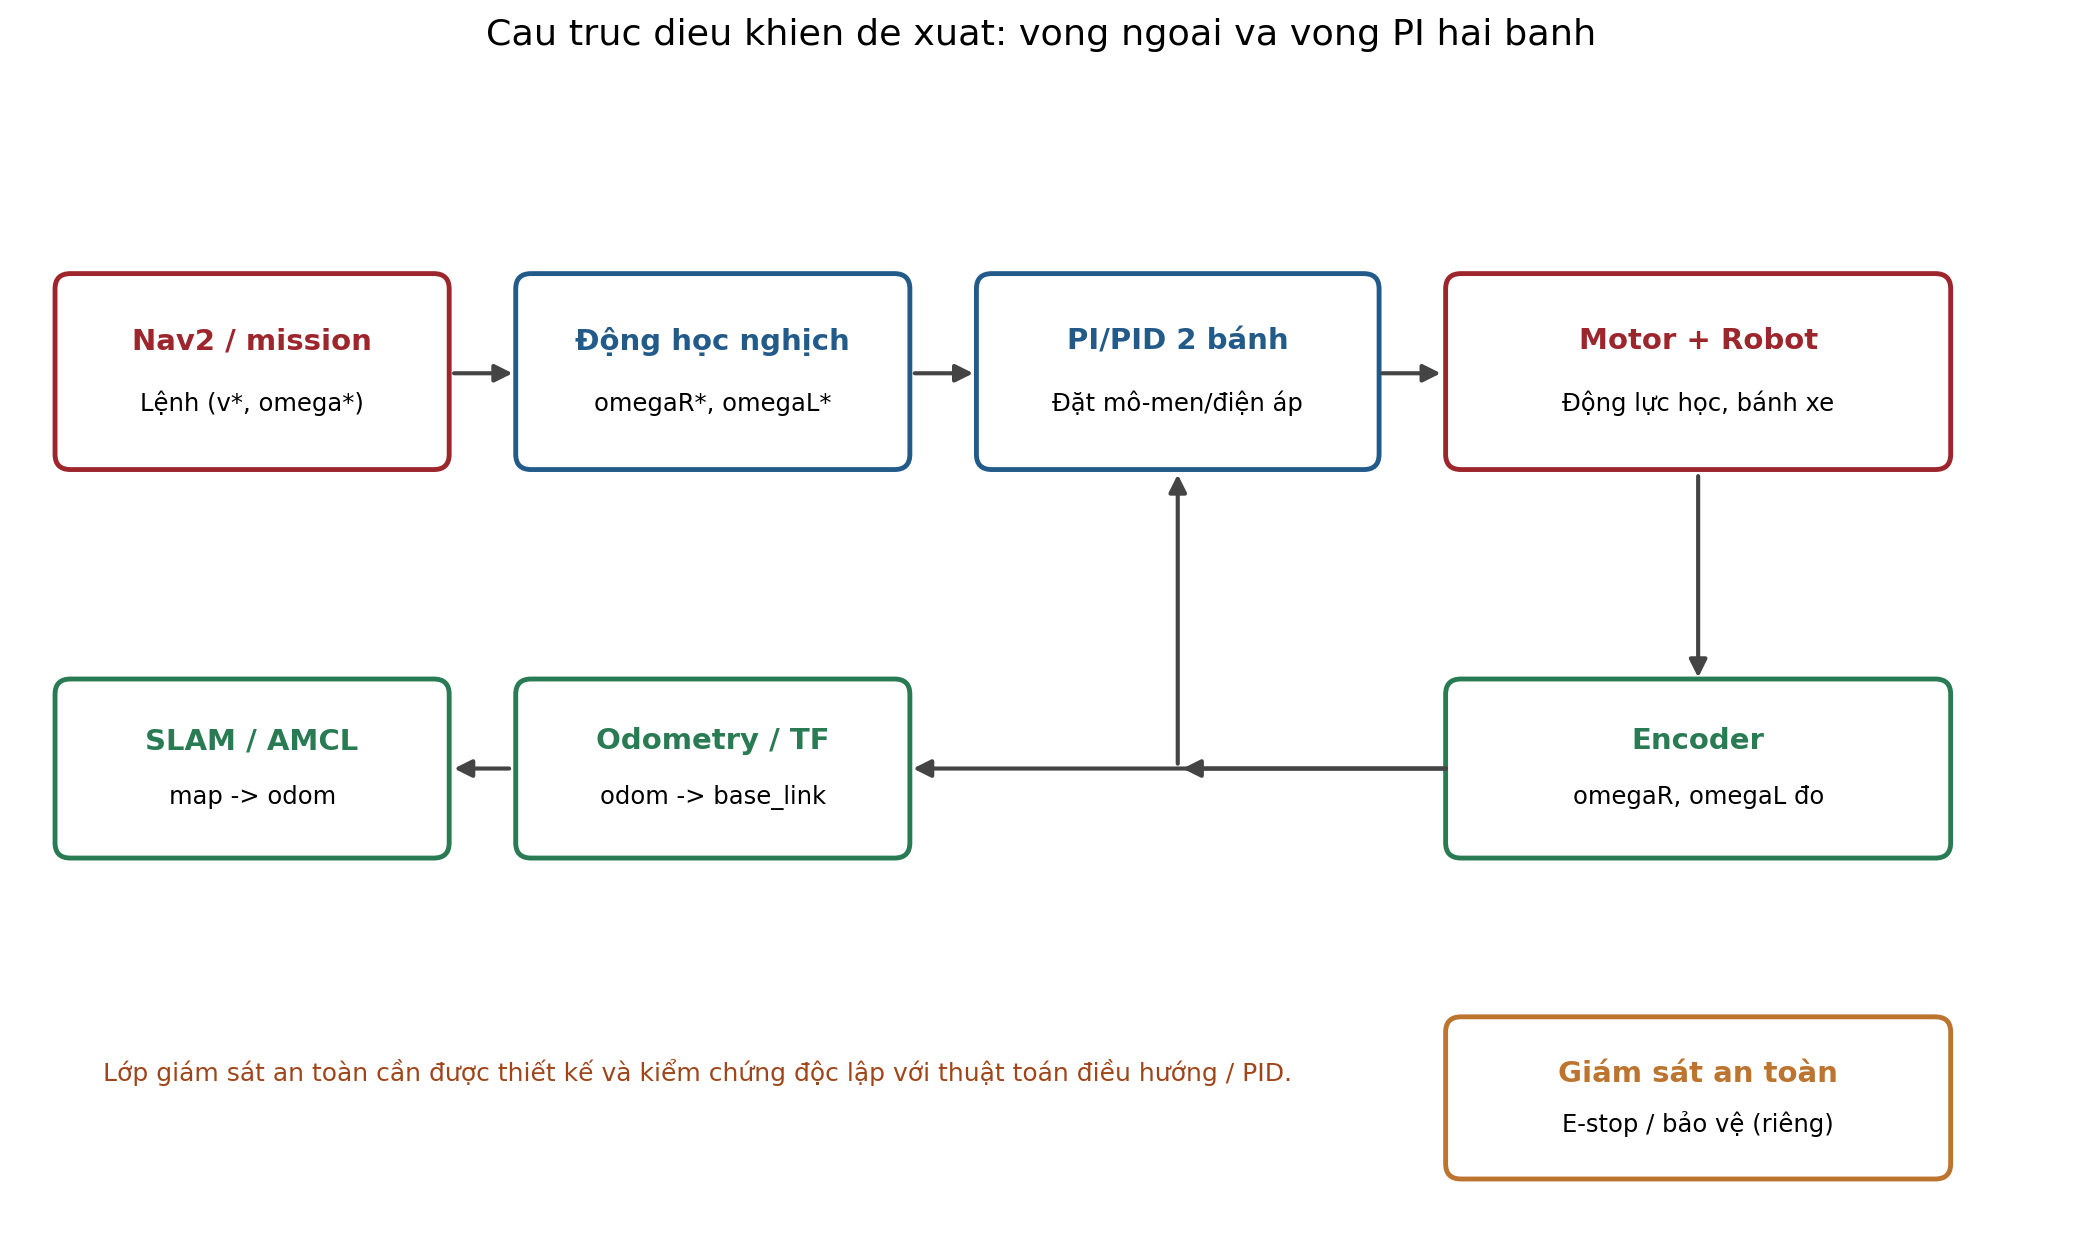
\includegraphics{assets/control_architecture.png}
\caption{Hình 2. Sơ đồ chức năng bộ điều khiển robot vi sai.}
\end{figure}

\textbf{Phân biệt ba mức điều khiển:} (1) vòng nhiệm vụ/định vị/điều
hướng quyết định đi đâu; (2) vòng tốc độ thân \(v,\omega\) hoặc lệnh vận
tốc bánh quyết định chuyển động; (3) vòng tốc độ motor/bánh dùng PI/PID
bám setpoint. PID điều tốc \textbf{không tự bảo đảm} sai số dừng 30 mm;
docking có thể cần điều khiển vị trí tinh chỉnh, marker và phép đo tại
trạm.

\subsection{4.2. Luật PID cho từng
bánh}\label{luux1eadt-pid-cho-tux1eebng-buxe1nh}

Đặt \(e_i(t)=\dot\varphi^*_i(t)-\dot\varphi_i(t)\), với \(i\in\{L,R\}\).
Bộ điều khiển PID liên tục:

\[
u_i(t)=K_{p,i}e_i(t)+K_{i,i}\int_0^t e_i(\tau)\,d\tau
+K_{d,i}\frac{de_i(t)}{dt}.
\]

Đầu ra \(u\) có thể là yêu cầu mô-men, dòng điện hoặc PWM \textbf{tùy bộ
driver}. Vì vậy các hệ số \(K_p,K_i,K_d\) có đơn vị và giá trị khác nhau
giữa các giao diện; tuyệt đối không chép một bộ tham số bất kỳ sang phần
cứng khác. Với bài toán điều tốc, PI thường là điểm bắt đầu hợp lý;
thành phần D không bắt buộc vì đạo hàm của encoder nhiễu.

Dạng rời rạc ở chu kỳ \(T_s\):

\[
I_i[k]=I_i[k-1]+T_s e_i[k],\qquad
D_i[k]\approx\frac{e_i[k]-e_i[k-1]}{T_s},
\]

\[
u_i[k]=K_p e_i[k]+K_i I_i[k]+K_d D_i[k],\qquad
u_{i,\rm out}[k]=\operatorname{sat}(u_i[k],u_{\min},u_{\max}).
\]

Nên lọc đạo hàm hoặc dùng đạo hàm của giá trị đo để tránh ``giật'' khi
đổi setpoint. Bắt buộc quản lý bão hòa và \textbf{anti-windup} (khóa
tích phân hoặc back-calculation khi actuator bão hòa). Thêm giới hạn gia
tốc / jerk của lệnh vận tốc, timeout mất lệnh, xử lý encoder lỗi và
chính sách dừng an toàn theo kiến trúc điều khiển được phê duyệt.

\subsection{4.3. Trình tự hiệu chỉnh
PID}\label{truxecnh-tux1ef1-hiux1ec7u-chux1ec9nh-pid}

\begin{enumerate}
\def\labelenumi{\arabic{enumi}.}
\tightlist
\item
  Kiểm tra dấu encoder, dấu lệnh motor, giới hạn bánh, độ phân giải
  encoder, đúng tỷ số truyền và cách tính rad/s. Đảm bảo không có
  \textbf{hai vòng điều khiển tốc độ cùng tranh quyền}: driver motor có
  thể đã tích hợp PID/FOC, ROS 2 chỉ cần phát vận tốc đặt.
\item
  Thực hiện mô hình hóa một bánh hoặc thử vận tốc thấp trong môi trường
  thử nghiệm an toàn, đặt \(K_i=K_d=0\), tăng \(K_p\) từ nhỏ để kiểm tra
  phản ứng; không áp dụng bộ PID chưa hiệu chỉnh trực tiếp cho robot tải
  nặng trong khu vực có người.
\item
  Bổ sung \(K_i\) từ nhỏ để giảm sai số xác lập khi có tải; hạn chế tích
  phân khi bão hòa hoặc mất tiếp xúc mặt sàn.
\item
  Chỉ bổ sung \(K_d\) nếu có nhu cầu điều chỉnh quá độ và dữ liệu tốc độ
  đủ sạch; lọc tín hiệu đạo hàm.
\item
  Kiểm tra độc lập bánh trái/bánh phải, cả hai bánh cùng chạy, vận tốc
  tiến--quay kết hợp, tải 20 kg, quãng dừng và ảnh hưởng khi giảm điện
  áp pin. Sau đó mới xem xét điều khiển docking và navigation toàn hệ
  thống.
\end{enumerate}

\textbf{Không có cơ sở để tuyên bố bộ \(K_p,K_i,K_d\) cuối cùng nếu chưa
có thông số điện--cơ và log thử nghiệm.} Các giá trị trong script Python
kèm theo chỉ dùng tái lập ví dụ số, không dùng như cấu hình sản phẩm.

\subsection{4.4. Demo mô phỏng số có thể tái
lập}\label{demo-muxf4-phux1ecfng-sux1ed1-cuxf3-thux1ec3-tuxe1i-lux1eadp}

Script
\href{../examples/simulate_diff_drive_pi.py}{\texttt{../examples/simulate\_diff\_drive\_pi.py}}
sử dụng mô hình quán tính 2 bánh nêu tại §3.2, cản nhớt và cản lăn giả
định, cùng PI tốc độ độc lập hai bánh. Nó mô phỏng profile tăng tốc
\(0\to1,2\) m/s, giữ tốc độ rồi giảm về 0. Các điều kiện minh họa thêm:
\(J_w=0,012\) kg·m² mỗi bánh, giới hạn mô-men bánh \(8\) N·m, hệ số điều
khiển PI khởi tạo \(K_p=1,1\), \(K_i=3,0\), bước tích phân 5 ms. Đây
\textbf{không} phải dữ liệu đo từ Gazebo hoặc robot thật.

\begin{figure}
\centering
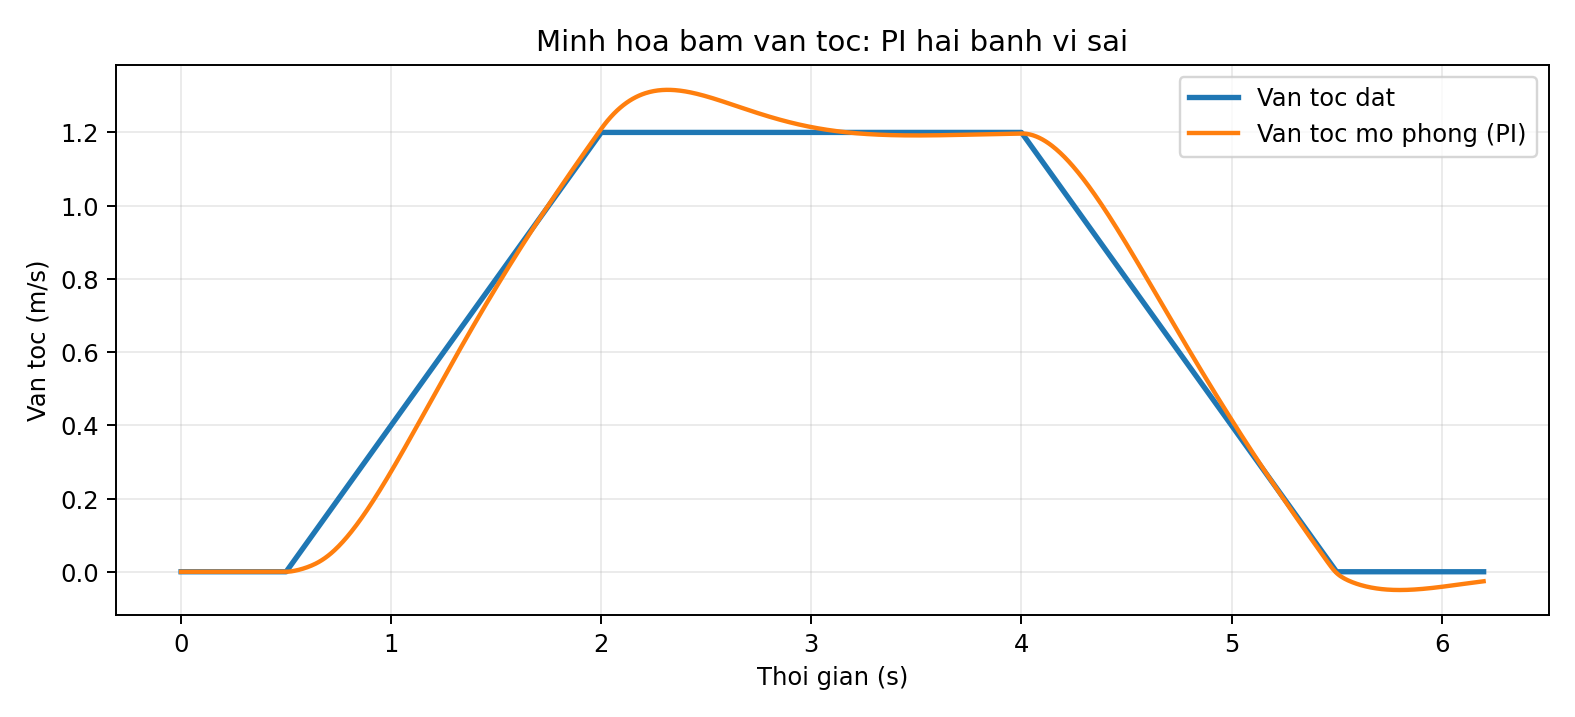
\includegraphics{assets/speed_response.png}
\caption{Hình 3. Minh họa lệnh tốc độ và tốc độ mô phỏng bằng PI hai
bánh.}
\end{figure}

\begin{figure}
\centering
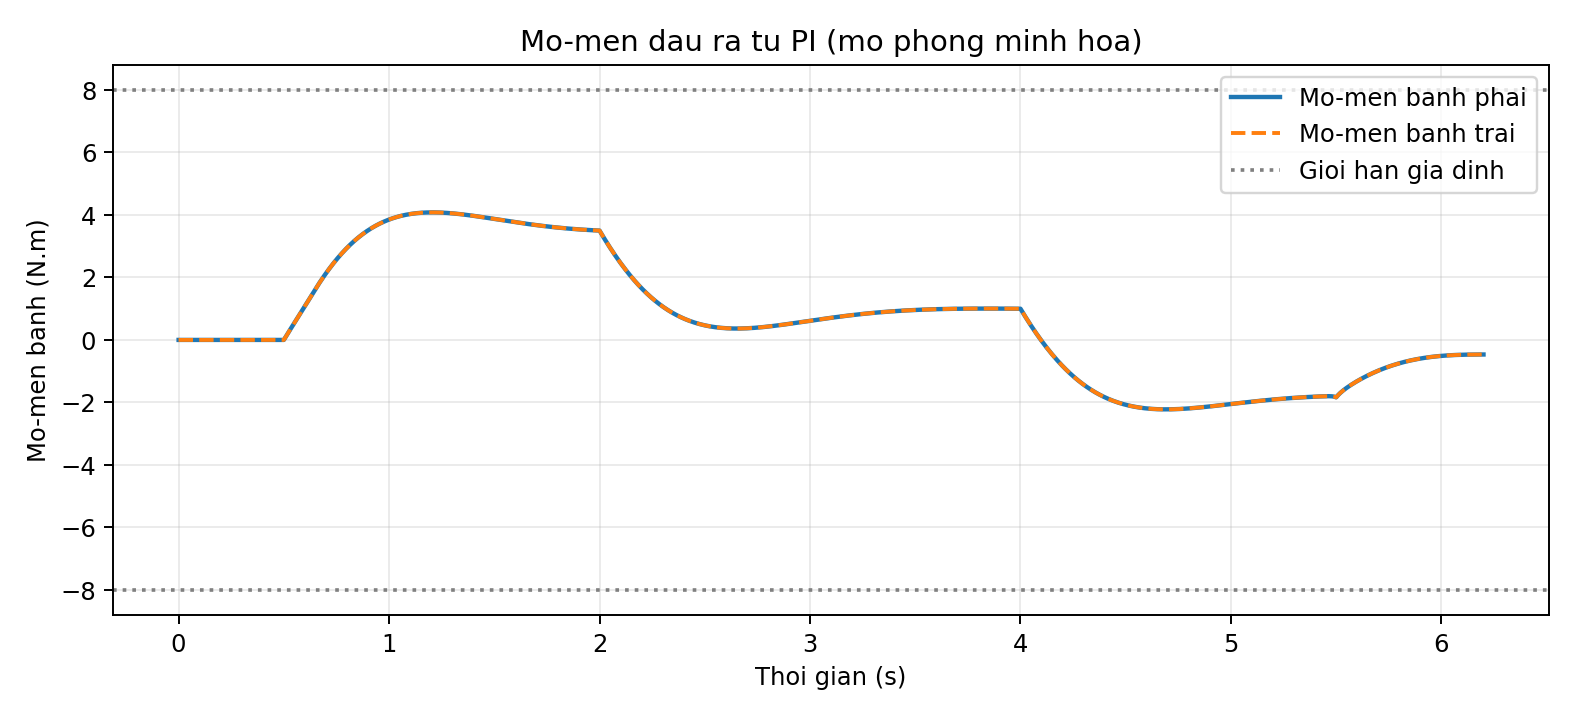
\includegraphics{assets/wheel_torque_response.png}
\caption{Hình 4. Mô-men bánh theo thời gian trong mô phỏng minh họa.}
\end{figure}

Đã chạy kiểm tra số: động học thuận/nghịch cho ra lại \((v,\omega)\) đã
đặt; mô hình tốc độ duy trì trung bình khoảng \textbf{1,196 m/s} trong
đoạn giữ lệnh 1,2 m/s; đầu ra mô-men không vượt ngưỡng bão hòa
\textbf{giả định} 8 N·m. Kết quả này chỉ chứng minh script hoạt động
theo mô hình đơn giản, \textbf{không chứng minh} yêu cầu khách hàng đã
đạt, đặc biệt là sai số docking, an toàn tránh người, quãng đường thực
và thời gian pin 4 giờ.

\subsection{4.5. Đồ thị mô phỏng số mở rộng và dữ liệu tái
lập}\label{ux111ux1ed3-thux1ecb-muxf4-phux1ecfng-sux1ed1-mux1edf-rux1ed9ng-vuxe0-dux1eef-liux1ec7u-tuxe1i-lux1eadp}

Ngoài bài thử tăng tốc--giữ tốc--giảm tốc ở §4.4, nhóm bổ sung một loạt
kịch bản minh họa \textbf{khác} trong script
\href{../examples/simulate_extended_plots.py}{\texttt{../examples/simulate\_extended\_plots.py}}:
đi thẳng rồi vào cua, quay tại chỗ, so sánh P với PI dưới nhiễu tải giả
định, và điều hướng đến bốn tọa độ giả định A→B→C→D. Kết quả có dữ liệu
CSV đi kèm; tham số, giới hạn, ngưỡng đạt được ghi đầy đủ trong
\href{03_bieu_do_mo_phong_mo_rong.md}{\texttt{03\_bieu\_do\_mo\_phong\_mo\_rong.md}}.

\begin{figure}
\centering
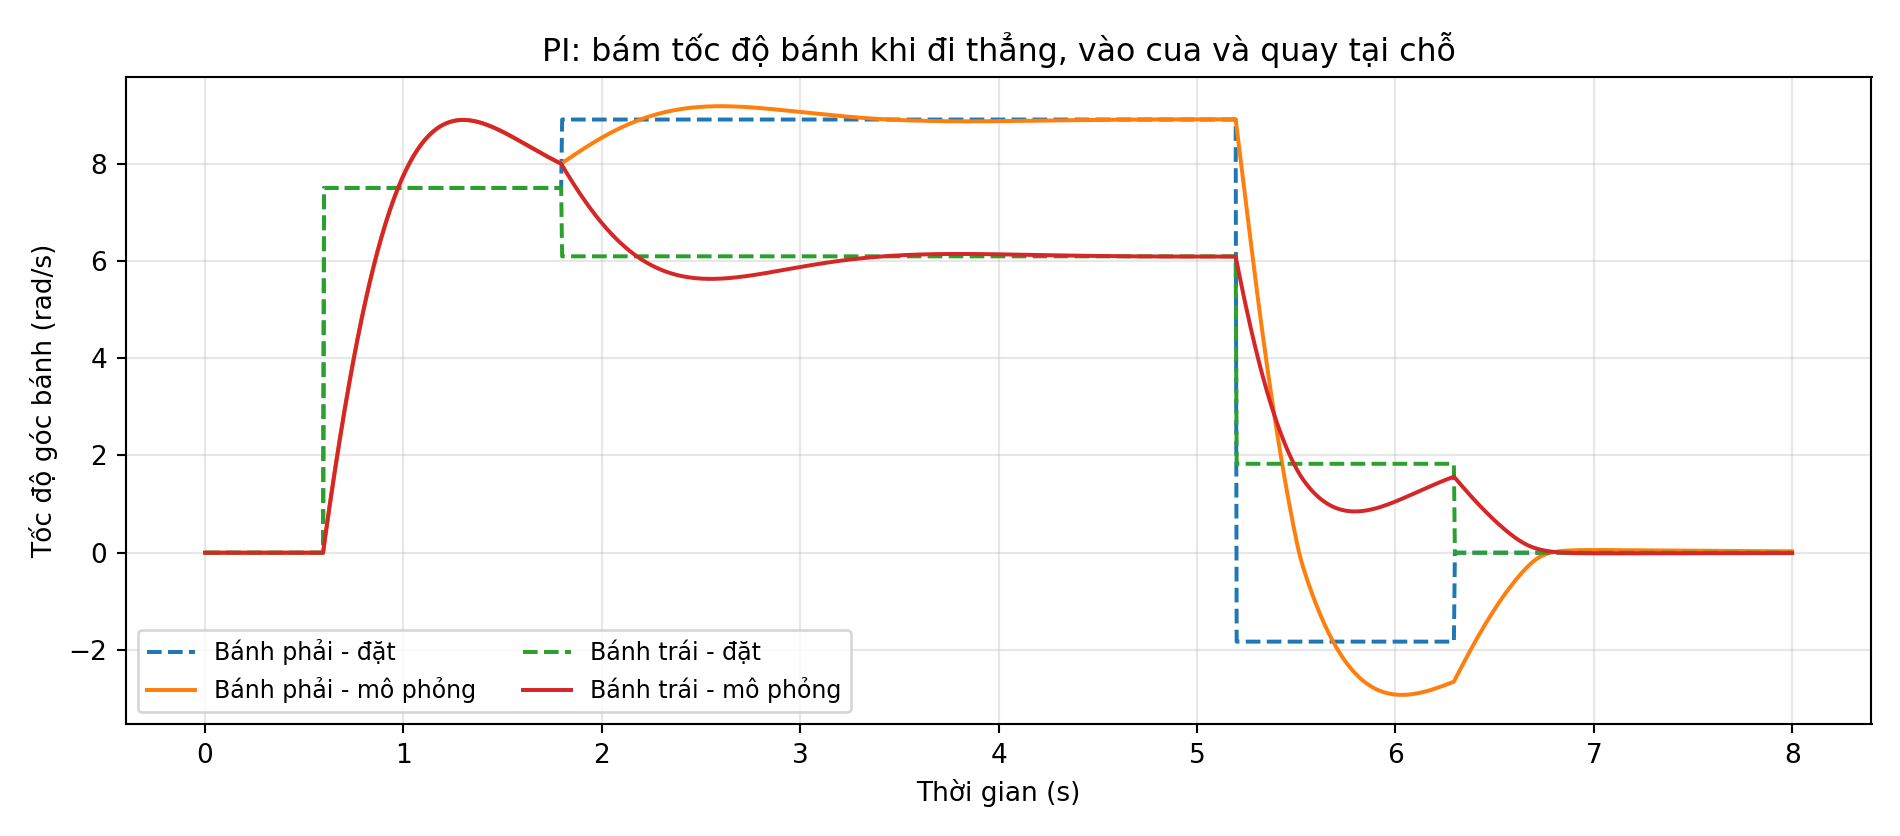
\includegraphics{assets/extended_wheel_speed_tracking.png}
\caption{Bám tốc độ góc hai bánh trong nhiều chế độ chuyển động.}
\end{figure}

\begin{figure}
\centering
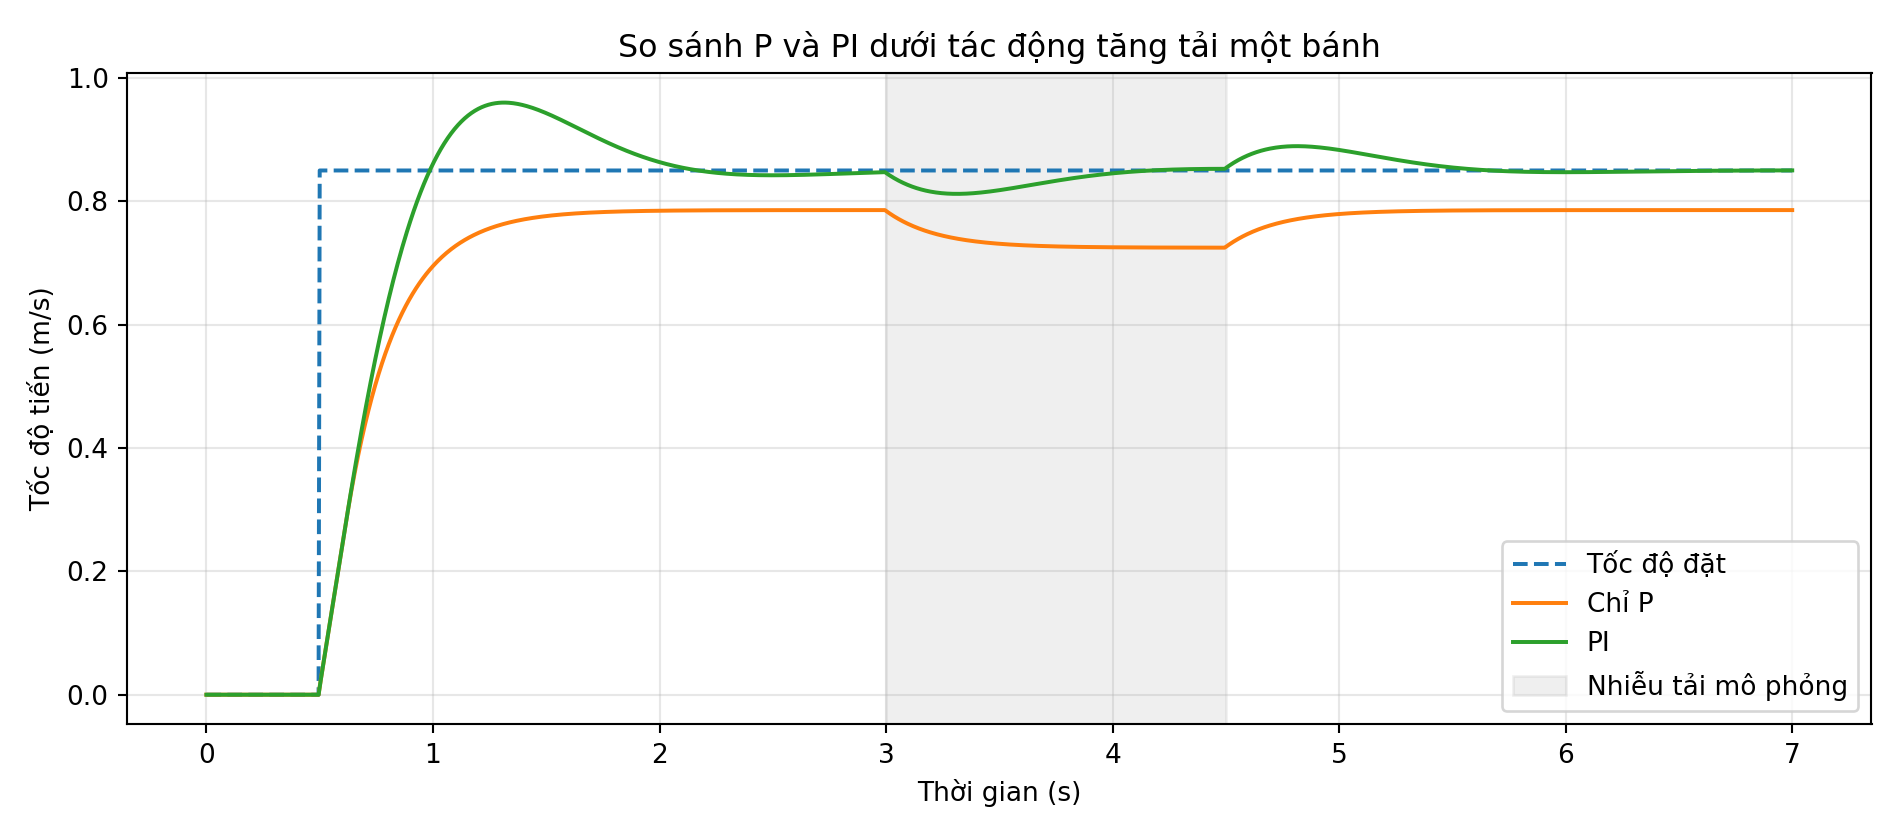
\includegraphics{assets/extended_p_vs_pi_disturbance.png}
\caption{So sánh điều khiển P và PI có nhiễu tải mô phỏng.}
\end{figure}

\begin{figure}
\centering
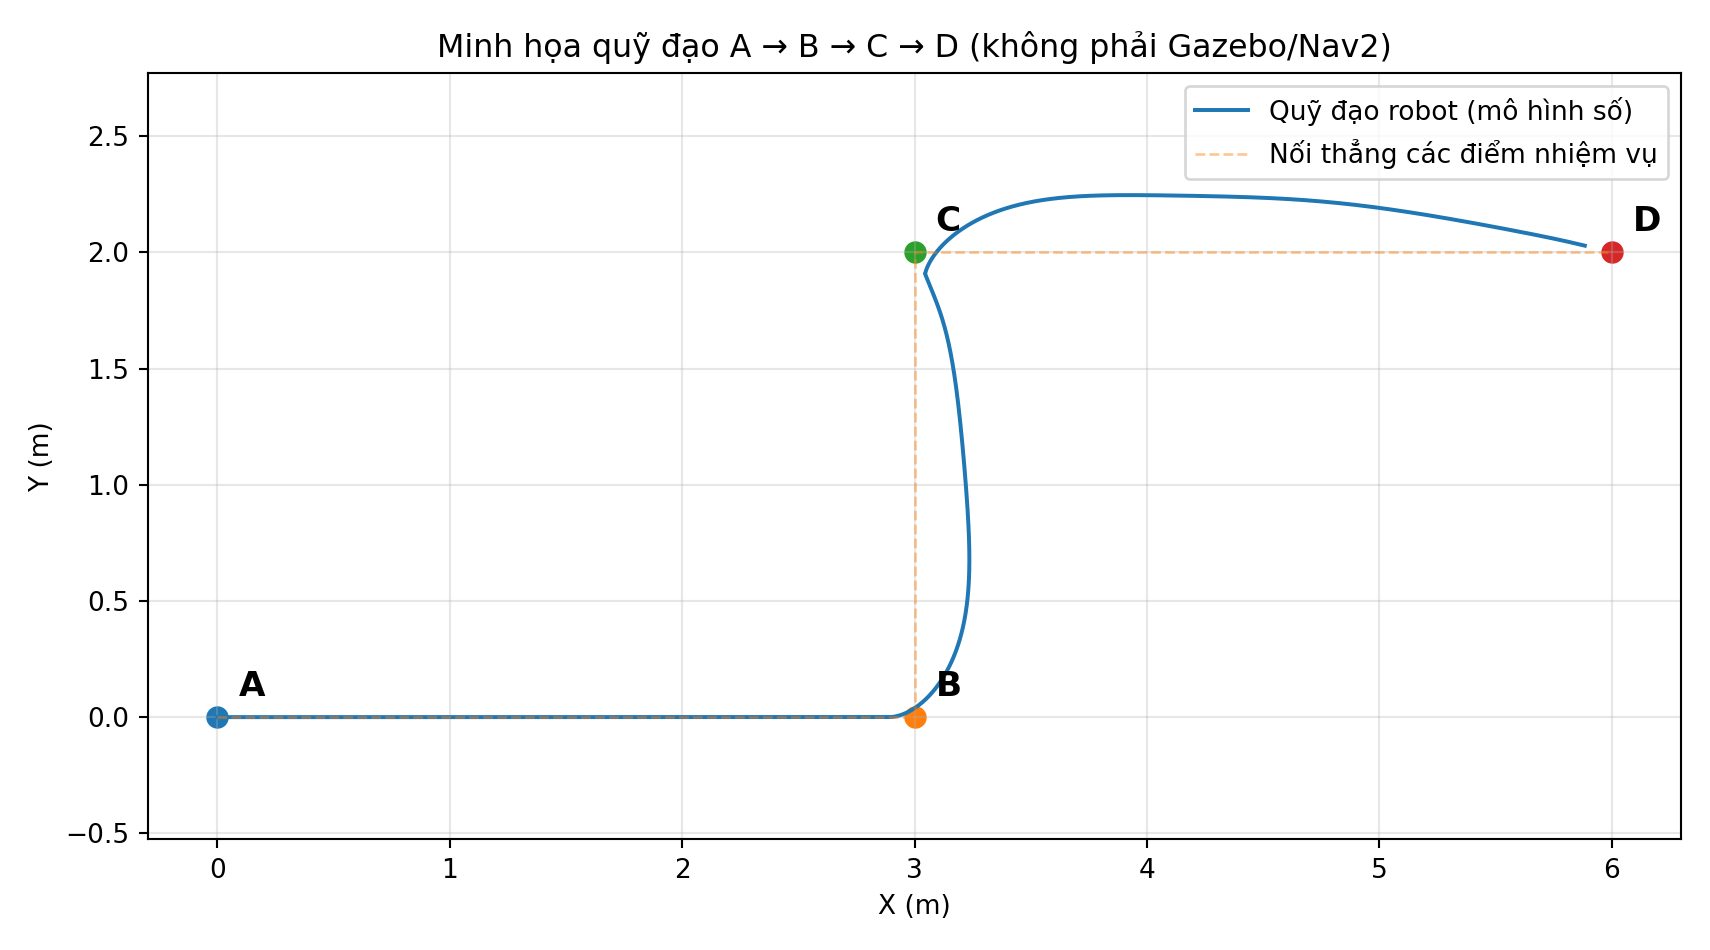
\includegraphics{assets/extended_waypoint_abcd.png}
\caption{Quỹ đạo minh họa nối điểm A → B → C → D bằng bộ điều khiển đơn
giản trong Python.}
\end{figure}

Các biểu đồ mới \textbf{không đo trên Gazebo, Nav2 hay robot thật}. Bộ
điều khiển đi theo waypoint là phương pháp kiểm tra động học ở mức số,
không phải chứng minh hệ robot đã chạy trong nhà máy. Chuyển waypoint
khi khoảng cách còn \textless{} 0,12 m chỉ là ngưỡng mô phỏng,
\textbf{không phải} minh chứng đạt sai số dừng 30 mm.

\section{5. Áp dụng vào ROS 2 Jazzy, Gazebo và mô hình URDF của
nhóm}\label{uxe1p-dux1ee5ng-vuxe0o-ros-2-jazzy-gazebo-vuxe0-muxf4-huxecnh-urdf-cux1ee7a-nhuxf3m}

\subsection{5.1. Các tham số phải kiểm tra thống
nhất}\label{cuxe1c-tham-sux1ed1-phux1ea3i-kiux1ec3m-tra-thux1ed1ng-nhux1ea5t}

\begin{longtable}[]{@{}
  >{\raggedright\arraybackslash}p{(\columnwidth - 4\tabcolsep) * \real{0.3333}}
  >{\raggedright\arraybackslash}p{(\columnwidth - 4\tabcolsep) * \real{0.3333}}
  >{\raggedright\arraybackslash}p{(\columnwidth - 4\tabcolsep) * \real{0.3333}}@{}}
\toprule\noalign{}
\begin{minipage}[b]{\linewidth}\raggedright
Phần
\end{minipage} & \begin{minipage}[b]{\linewidth}\raggedright
Tệp hoặc dữ liệu cần đối chiếu
\end{minipage} & \begin{minipage}[b]{\linewidth}\raggedright
Lỗi phổ biến
\end{minipage} \\
\midrule\noalign{}
\endhead
\bottomrule\noalign{}
\endlastfoot
URDF/Xacro & \texttt{wheel\_radius}, vị trí tâm bánh, joint axis, mass,
inertia & Lấy bề rộng thân thay cho wheel separation \\
Gazebo DiffDrive & \texttt{\textless{}wheel\_radius\textgreater{}},
\texttt{\textless{}wheel\_separation\textgreater{}}, tên
\texttt{left\_joint/right\_joint} & Sai dấu hoặc trùng tên joint \\
ros2\_control & \texttt{wheel\_radius}, \texttt{wheel\_separation},
command/state interfaces & Hai node cùng điều khiển motor \\
Odometry/TF & \texttt{/odom}, \texttt{/tf},
\texttt{map\ →\ odom\ →\ base\_link} & Nhiều publisher cùng phát
odom→base\_link \\
Sensor & Encoder, IMU, LiDAR và timestamp & Tốc độ encoder sai hệ số /
đơn vị \\
PID driver & Đầu vào là PWM, dòng điện, mô-men hay vận tốc & Gán Kp/Ki
từ mô hình torque sang PWM \\
\end{longtable}

Với Gazebo Harmonic, cần kiểm tra plugin Gazebo hiện có đã điều khiển
vận tốc bánh ở mức trừu tượng hay thật sự sử dụng mô hình mô-men/quán
tính motor. Nếu chỉ là plugin DiffDrive nhận vận tốc, biểu đồ động lực
và PI motor trong Python không thể được coi là bằng chứng Gazebo đã kiểm
thử lực/mô-men. Nếu dùng \texttt{ros2\_control} với interface vận tốc,
bộ điều khiển vi sai có thể chỉ chuyển \(v,\omega\) sang lệnh vận tốc
joint; vòng PID thấp hơn có thể nằm trong driver hoặc trong một tầng
khác.

\subsection{5.2. Kịch bản kiểm thử nhóm nên chạy và lưu bằng
chứng}\label{kux1ecbch-bux1ea3n-kiux1ec3m-thux1eed-nhuxf3m-nuxean-chux1ea1y-vuxe0-lux1b0u-bux1eb1ng-chux1ee9ng}

\begin{longtable}[]{@{}
  >{\raggedright\arraybackslash}p{(\columnwidth - 4\tabcolsep) * \real{0.3333}}
  >{\raggedright\arraybackslash}p{(\columnwidth - 4\tabcolsep) * \real{0.3333}}
  >{\raggedright\arraybackslash}p{(\columnwidth - 4\tabcolsep) * \real{0.3333}}@{}}
\toprule\noalign{}
\begin{minipage}[b]{\linewidth}\raggedright
Mã
\end{minipage} & \begin{minipage}[b]{\linewidth}\raggedright
Kịch bản
\end{minipage} & \begin{minipage}[b]{\linewidth}\raggedright
Dữ liệu đầu ra phải lưu
\end{minipage} \\
\midrule\noalign{}
\endhead
\bottomrule\noalign{}
\endlastfoot
KT-01 & Hai bánh tốc độ bằng nhau → đi thẳng & \texttt{/cmd\_vel},
\texttt{/odom}, \texttt{/joint\_states}, đường đi \\
KT-02 & Hai bánh quay ngược chiều → quay tại chỗ & Sai lệch yaw, quỹ
đạo, tốc độ bánh \\
KT-03 & Lệnh \((v,\omega)\) kết hợp → chạy cung tròn & Bán kính lý
thuyết và thực nghiệm \\
PI-01 & Bám profile tốc độ khi không tải & Rise time, overshoot, sai số
xác lập, torque/PWM \\
PI-02 & Bám profile với tải 20 kg & Tốc độ, dòng/mô-men, nhiệt độ, giới
hạn \\
PI-03 & Thử mất lệnh / phản hồi encoder lỗi & Log sự kiện và hành vi an
toàn \\
SYS-01 & Nhiệm vụ A → B → C → D & Thời gian, kết quả từng waypoint, nhật
ký Nav2 \\
SYS-02 & Dừng tại trạm & Sai số x-y-yaw đo theo mốc đã chốt \\
\end{longtable}

\textbf{Điều kiện nghiệm thu chưa đầy đủ:} tốc độ 1,2 m/s phải được kiểm
tra dưới điều kiện thử được duyệt; sai số dừng \(<30\) mm cần mốc đo và
nhiều lần lặp; an toàn người/vật cản không thể kết luận chỉ từ PID; thời
gian pin 4 giờ cần thử theo duty cycle thực tế. Các chức năng an toàn
phải được đánh giá và kiểm chứng riêng.

\subsection{5.3. Phân chia đầu việc để nhập tài liệu vào dự
án}\label{phuxe2n-chia-ux111ux1ea7u-viux1ec7c-ux111ux1ec3-nhux1eadp-tuxe0i-liux1ec7u-vuxe0o-dux1ef1-uxe1n}

Tài liệu được lưu tại \texttt{research/diff\_drive\_pid/docs/} trong
repository nhóm. Khi nhận được mã nguồn/ảnh Gazebo thật của nhóm, bổ
sung ảnh tại \texttt{docs/control/assets/} và thay các giả định bằng số
đọc được từ URDF, cấu hình controller, CAD và log. Gắn commit/tag và dẫn
nguồn đến đúng tệp thay vì dán ảnh không có xuất xứ. Không đưa kết quả
demo Python vào mục ``Kết quả Gazebo'' nếu chưa chạy thật.

\section{6. Kết quả mô phỏng số và phân tích đồ
thị}\label{kux1ebft-quux1ea3-muxf4-phux1ecfng-sux1ed1-vuxe0-phuxe2n-tuxedch-ux111ux1ed3-thux1ecb}

\subsection{6.1. Ma trận thí nghiệm và bằng
chứng}\label{ma-trux1eadn-thuxed-nghiux1ec7m-vuxe0-bux1eb1ng-chux1ee9ng}

Các đồ thị của chương này được tái tạo bằng \textbf{Python}, sử dụng
đúng giả định tại Bảng thông số ở Chương 1 và có dữ liệu CSV/JSON đi
kèm. Code MATLAB trong thư mục \texttt{matlab/} tái hiện những thí
nghiệm tương đương nhưng \textbf{chưa được chạy trong MATLAB tại thời
điểm xuất tài liệu}. Vì vậy ảnh \texttt{extended\_*.png} và
\texttt{python\_*.png} không được ghi là ảnh kết quả MATLAB, Gazebo hoặc
robot thật.

\begin{longtable}[]{@{}
  >{\raggedright\arraybackslash}p{(\columnwidth - 4\tabcolsep) * \real{0.3333}}
  >{\raggedright\arraybackslash}p{(\columnwidth - 4\tabcolsep) * \real{0.3333}}
  >{\raggedright\arraybackslash}p{(\columnwidth - 4\tabcolsep) * \real{0.3333}}@{}}
\toprule\noalign{}
\begin{minipage}[b]{\linewidth}\raggedright
Nhóm thử nghiệm
\end{minipage} & \begin{minipage}[b]{\linewidth}\raggedright
Hình trong báo cáo
\end{minipage} & \begin{minipage}[b]{\linewidth}\raggedright
Đại lượng đánh giá
\end{minipage} \\
\midrule\noalign{}
\endhead
\bottomrule\noalign{}
\endlastfoot
Tăng tốc, giữ và giảm tốc & Tốc độ và mô-men & Sai số tốc độ, giới
hạn \\
Đi thẳng, rẽ cong, quay tại chỗ & Vận tốc thân và hai bánh & Bám lệnh và
quỹ đạo \\
Sai số và quỹ đạo & Sai số hai bánh, đường XY & Quá độ và sai lệch \\
Nhiễu tải & Đường đáp ứng P/PI & Phản ứng khi tăng tải \\
A--B--C--D minh họa & Quỹ đạo và khoảng cách trạm & Thời gian chuyển
điểm \\
PI/PID lọc đạo hàm & Tốc độ và mô-men & Ảnh hưởng D và bão hòa \\
\end{longtable}

\subsection{6.2. Đi thẳng, rẽ cong và quay tại
chỗ}\label{ux111i-thux1eb3ng-rux1ebd-cong-vuxe0-quay-tux1ea1i-chux1ed7}

\begin{figure}
\centering
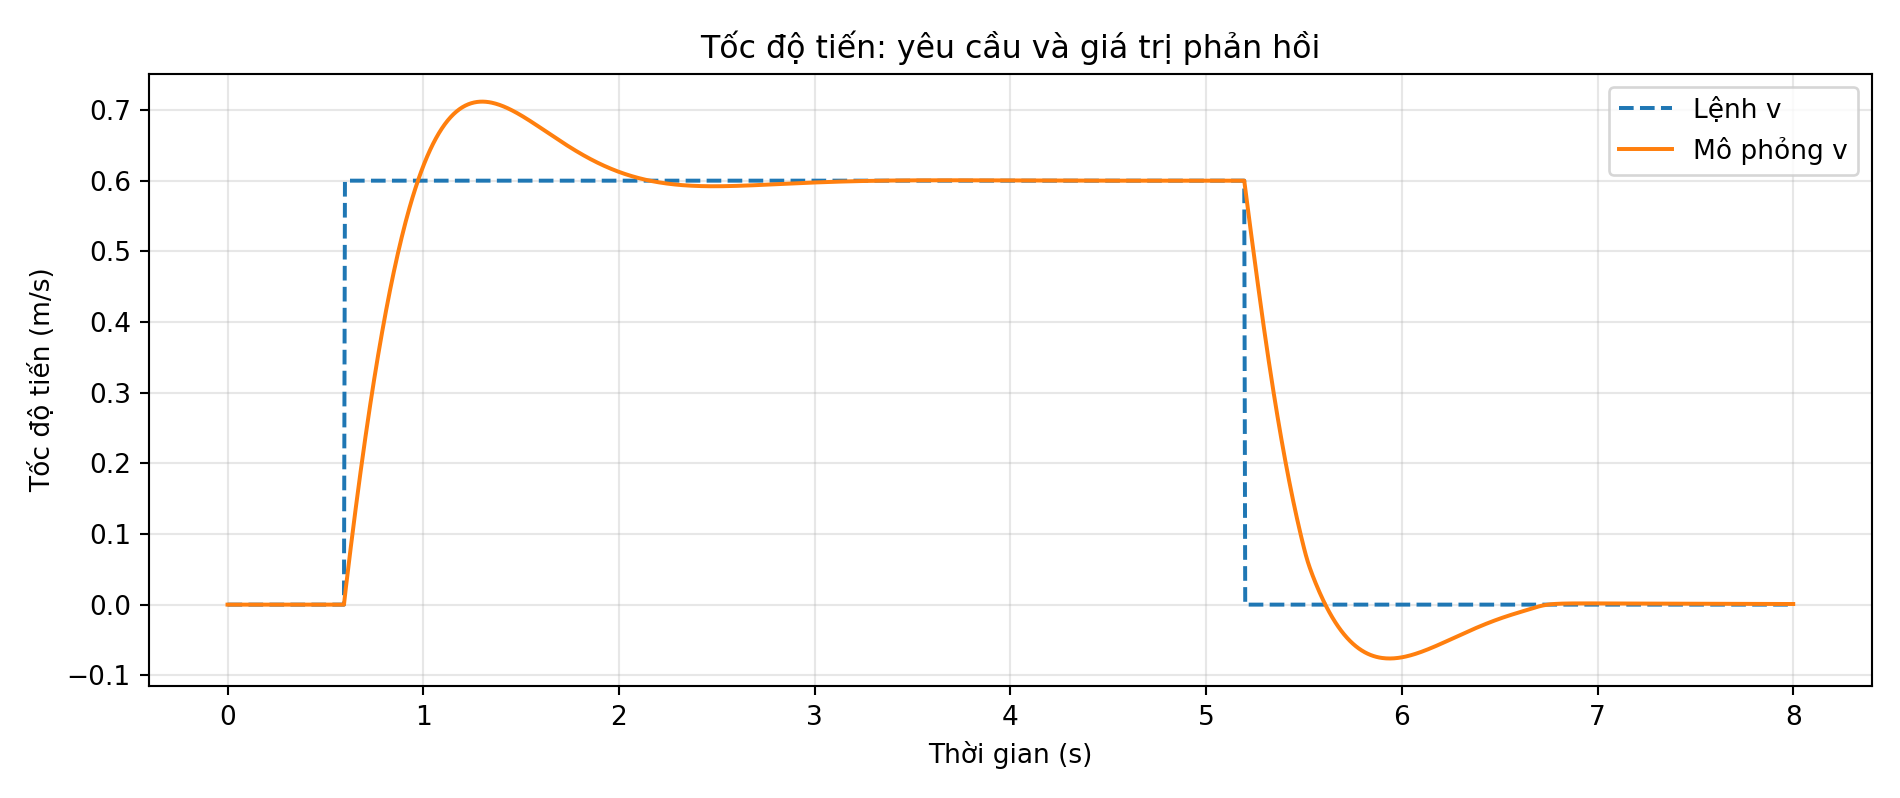
\includegraphics{assets/extended_body_linear_speed.png}
\caption{Vận tốc tiến khi đổi chế độ chuyển động --- mô phỏng số bằng
Python.}
\end{figure}

Vận tốc tiến đặt có các khoảng giữ lệnh 0,60 m/s và khoảng về 0 khi quay
tại chỗ; vận tốc thực phản ứng trễ do quán tính và giới hạn mô-men. Đây
là kết quả mô hình đơn giản trên nền phẳng, không có vật cản.

\begin{figure}
\centering
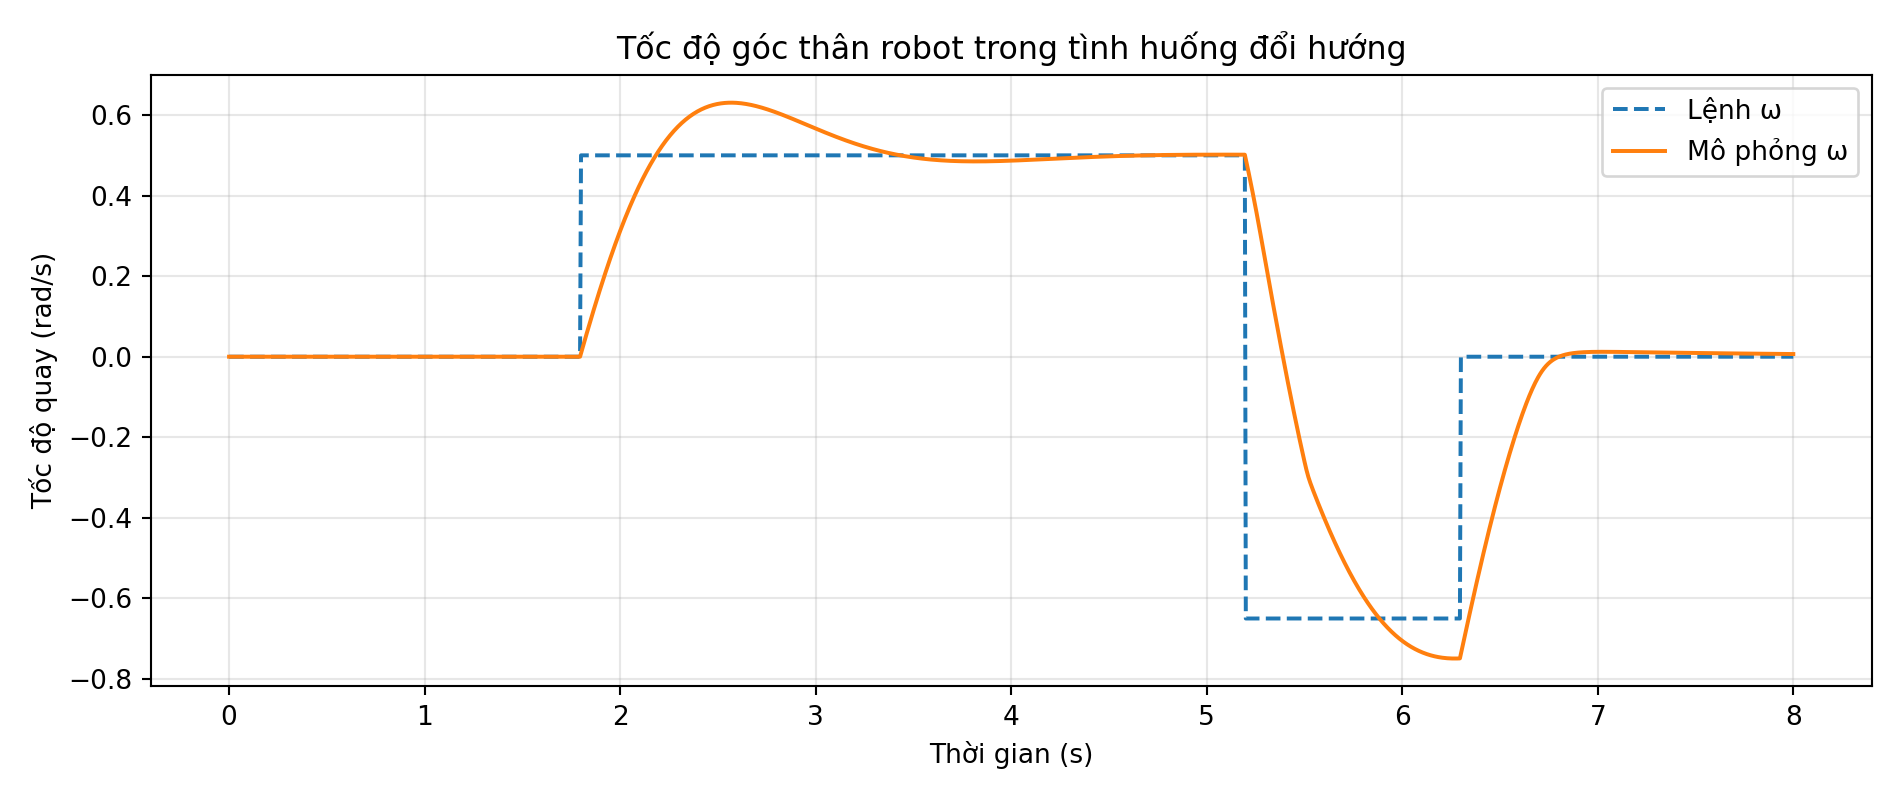
\includegraphics{assets/extended_body_yaw_rate.png}
\caption{Vận tốc quay thân khi đổi chế độ --- mô phỏng số bằng Python.}
\end{figure}

Ở đoạn quay trong hành lang, lệnh quay thân được quy đổi thành chênh
lệch tốc độ hai bánh. Đường phản hồi không trùng hoàn toàn với lệnh vì
vòng PI và quán tính tương đương. Chưa có kiểm chứng góc quay trên
Gazebo.

\begin{figure}
\centering
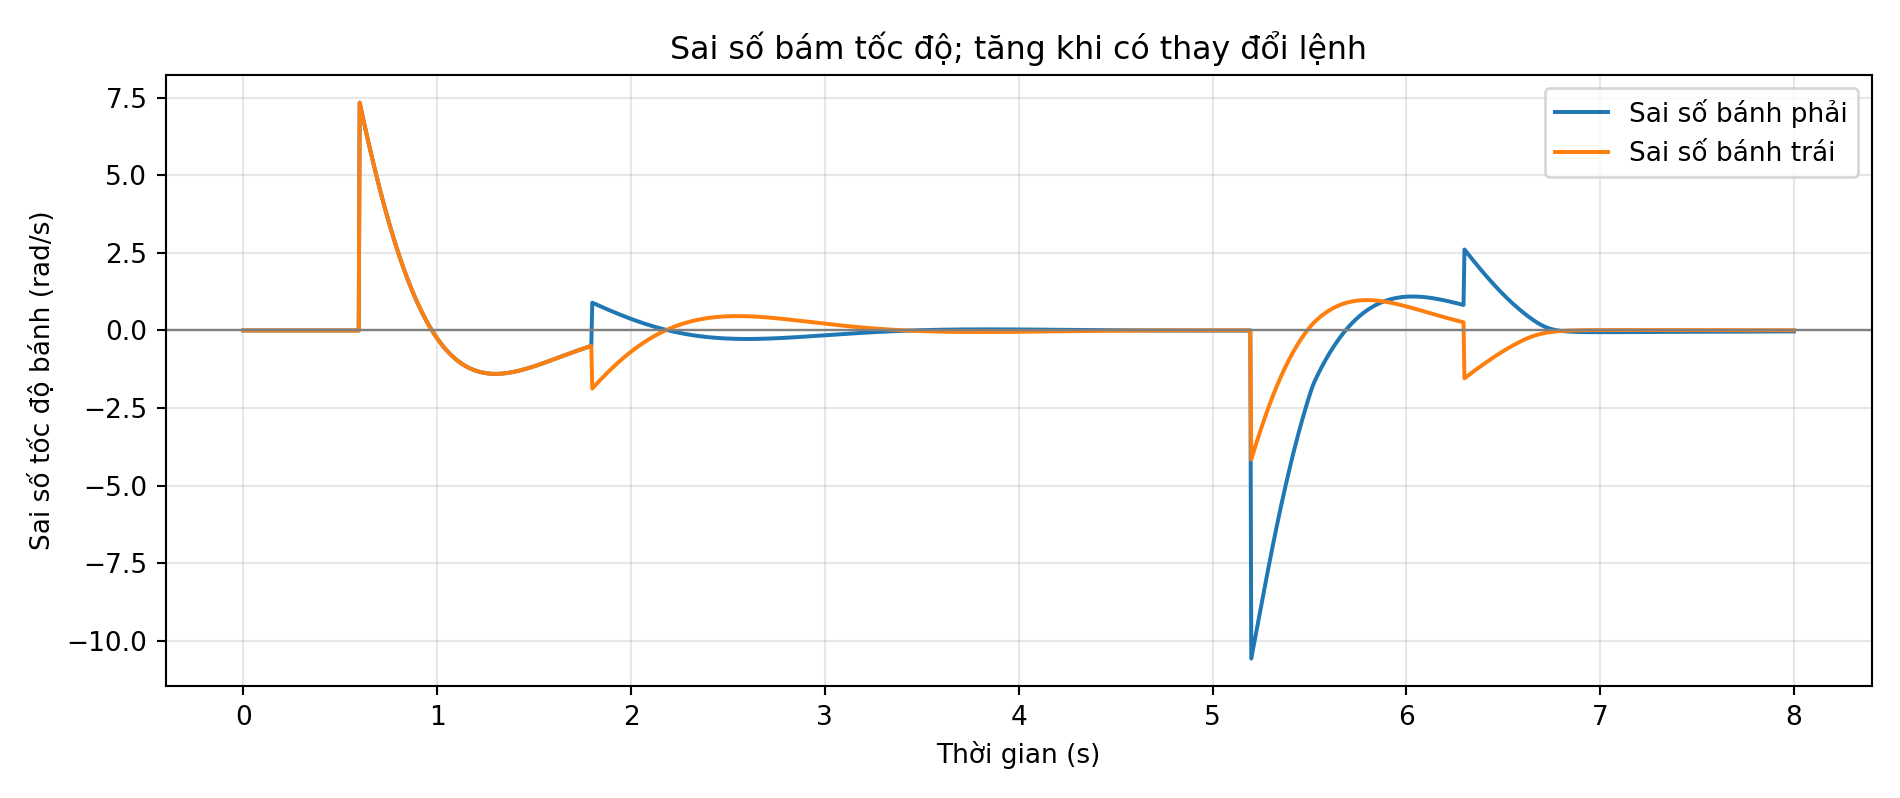
\includegraphics{assets/extended_wheel_error.png}
\caption{Sai số tốc độ bánh trái và bánh phải trong các chế độ.}
\end{figure}

Sai số lớn nhất thường xuất hiện ngay sau khi đặt lệnh thay đổi nhanh.
Cần kiểm tra cả sai số xác lập và quá độ; chỉ nhìn đường vận tốc tiến
không đủ để đánh giá hai vòng điều khiển bánh có cân bằng nhau hay
không.

\begin{figure}
\centering
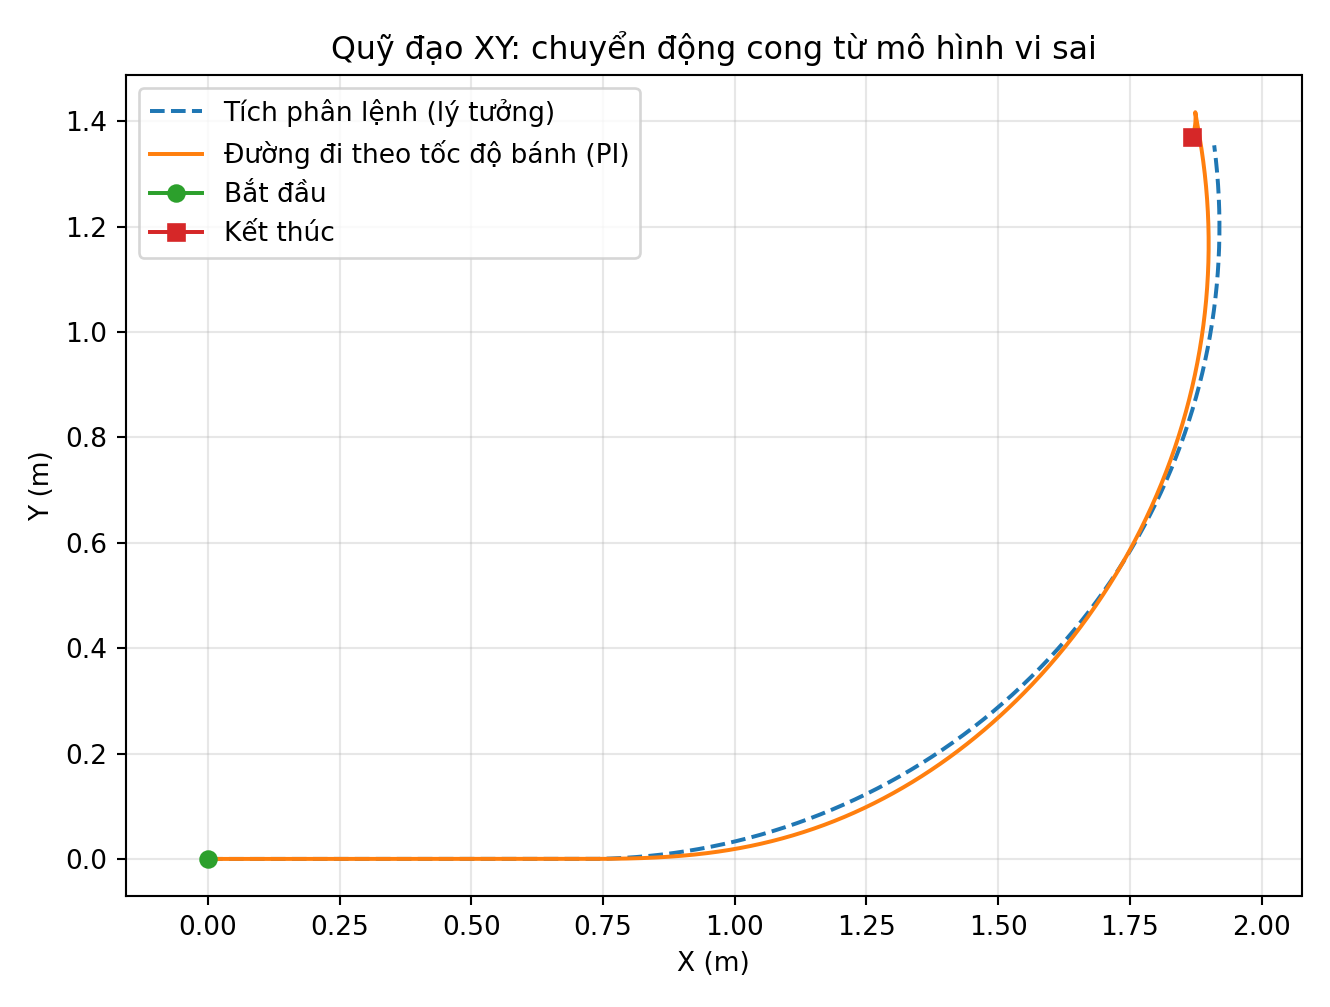
\includegraphics{assets/extended_turning_trajectory.png}
\caption{Quỹ đạo lý tưởng và quỹ đạo thực mô hình số trong pha đổi
hướng.}
\end{figure}

Sự lệch quỹ đạo giữa tích phân lệnh và tích phân vận tốc bánh mô phỏng
phản ánh hạn chế của vòng điều tốc khi lệnh thay đổi. Muốn đánh giá
chính xác cần có thông số bánh, khối lượng, quán tính và bản đồ kho
thật.

\begin{figure}
\centering
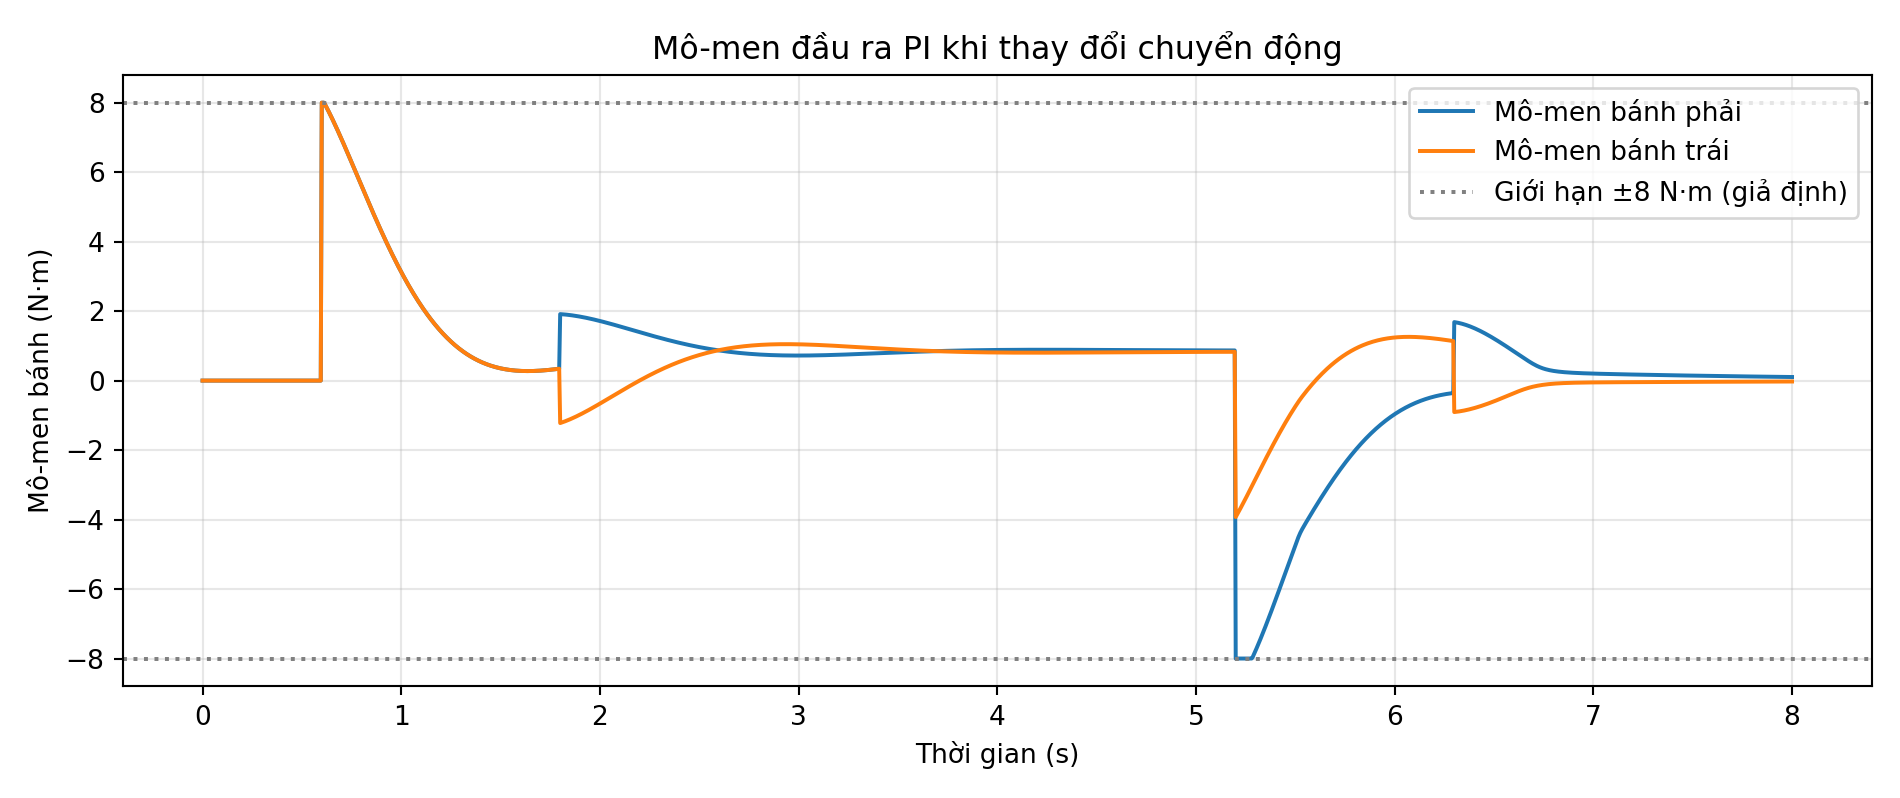
\includegraphics{assets/extended_wheel_torque.png}
\caption{Mô-men bánh trái và phải trong bài thử đổi hướng.}
\end{figure}

Mô-men được giới hạn trong ±8 N·m \textbf{theo giả định của mô hình},
không phải trị số liên tục/đỉnh của động cơ đã được mua. Với tỷ số
truyền và hiệu suất đã giả định, giá trị mô-men tại bánh phải được quy
đổi mới dùng để so sánh datasheet motor.

\subsection{6.3. So sánh P và PI khi có nhiễu
tải}\label{so-suxe1nh-p-vuxe0-pi-khi-cuxf3-nhiux1ec5u-tux1ea3i}

\begin{figure}
\centering
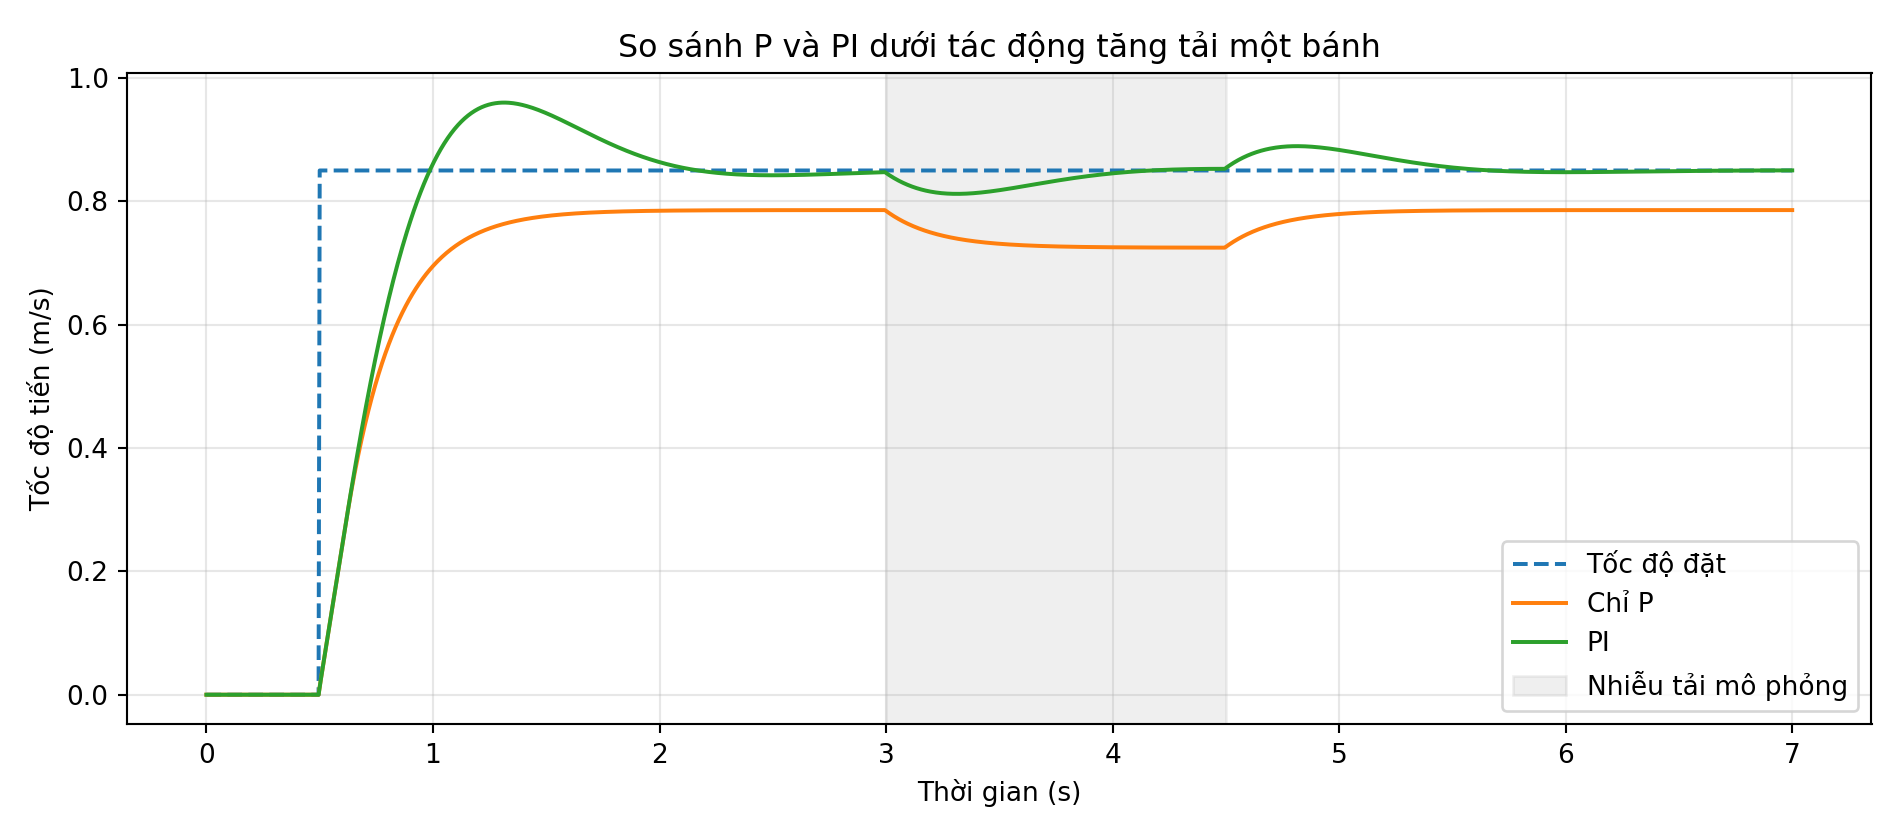
\includegraphics{assets/extended_p_vs_pi_disturbance.png}
\caption{So sánh P và PI khi thêm nhiễu mô-men ở bánh trái từ 3 đến 4,5
s.}
\end{figure}

Thí nghiệm tạo mô-men tải phụ 1,7 N·m tại bánh trái từ 3,0 đến 4,5 s.
Theo mô hình này, khâu I giúp giảm sai số kéo dài so với chỉ P nhưng có
thể tạo dao động hoặc quá độ khi nhiễu kết thúc. Đây không phải bằng
chứng bộ PI phù hợp nhất với robot thực mà chỉ là cách minh họa cơ chế
điều khiển.

\subsection{6.4. So sánh PI và PID có đạo hàm
lọc}\label{so-suxe1nh-pi-vuxe0-pid-cuxf3-ux111ux1ea1o-huxe0m-lux1ecdc}

\begin{figure}
\centering
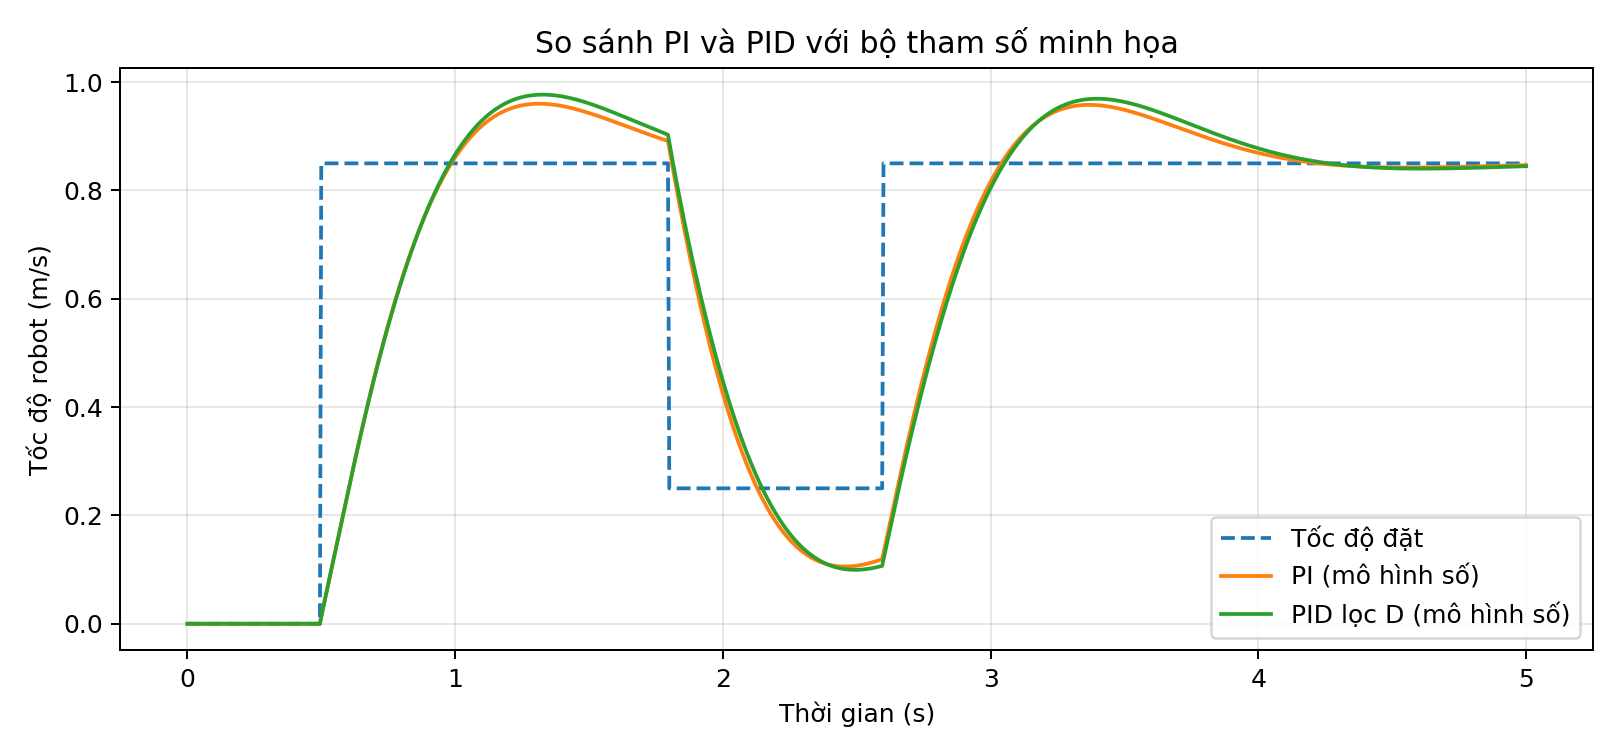
\includegraphics{assets/python_pi_vs_pid_speed.png}
\caption{Đáp ứng tốc độ PI và PID từ mô hình Python đối chiếu cấu trúc
MATLAB.}
\end{figure}

\begin{figure}
\centering
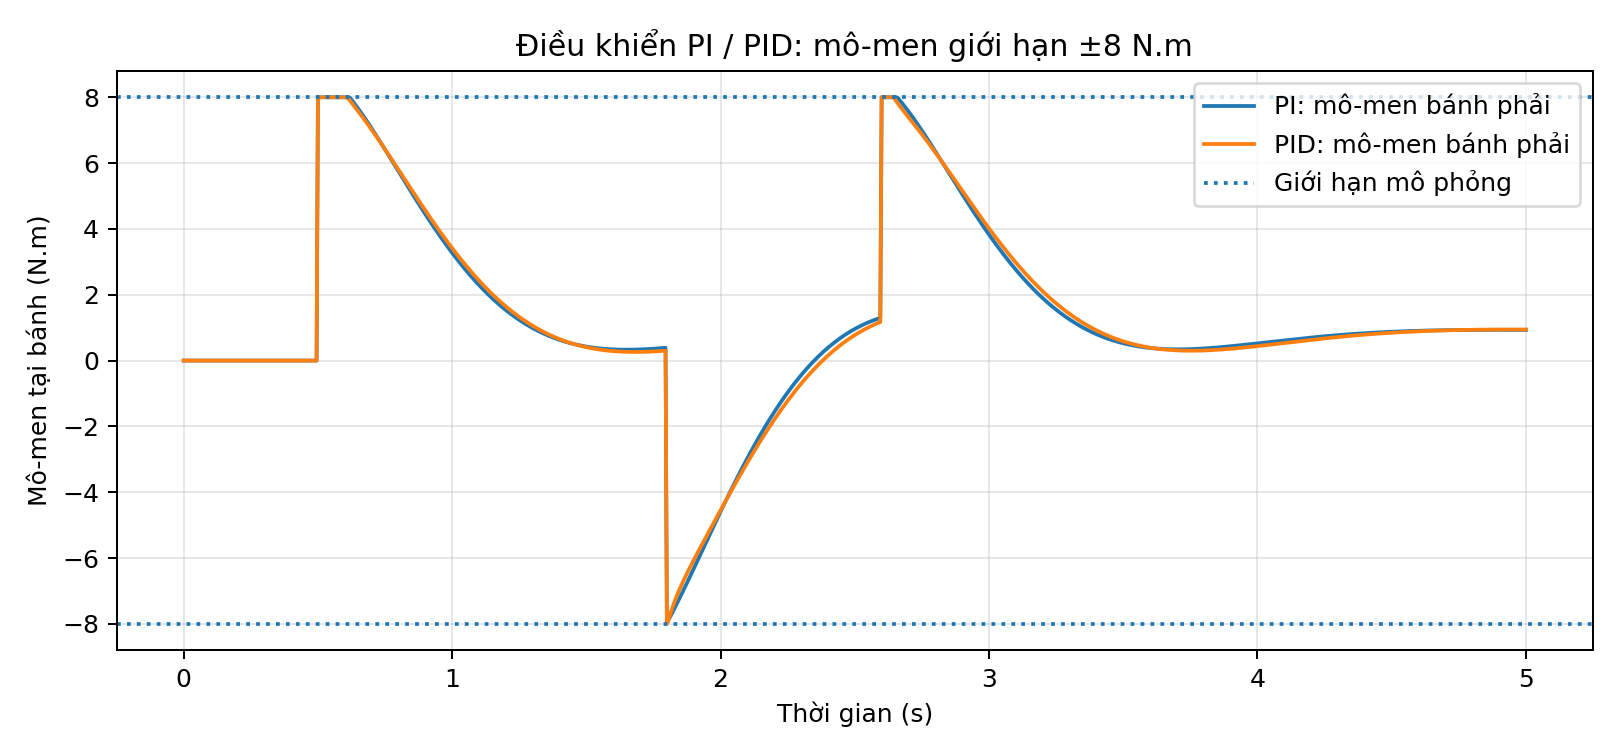
\includegraphics{assets/python_pi_vs_pid_torque.png}
\caption{Mô-men bánh phải khi dùng PI và PID, với giới hạn bão hòa minh
họa.}
\end{figure}

Cấu trúc PID sử dụng \textbf{đạo hàm của tốc độ đo} qua bộ lọc bậc nhất,
tránh xung đạo hàm khi thay đổi tốc độ đặt. Dùng \(K_p=1{,}1\),
\(K_i=3{,}0\), \(K_d=0{,}02\) và hằng số lọc \(0{,}04\) s trong ví dụ;
tất cả là hệ số \textbf{minh họa}. Trên toàn đoạn có lệnh khác 0, chương
trình đối chiếu Python cho RMSE tốc độ PI khoảng \textbf{0,211 m/s}, còn
PID khoảng \textbf{0,217 m/s}. Bộ PID này \textbf{không cải thiện RMSE
so với PI}, minh họa vì sao không thể khẳng định thêm thành phần D là
tốt hơn nếu chưa hiệu chỉnh.

\subsection{6.5. Mô phỏng nhiệm vụ A → B → C →
D}\label{muxf4-phux1ecfng-nhiux1ec7m-vux1ee5-a-b-c-d}

\begin{figure}
\centering
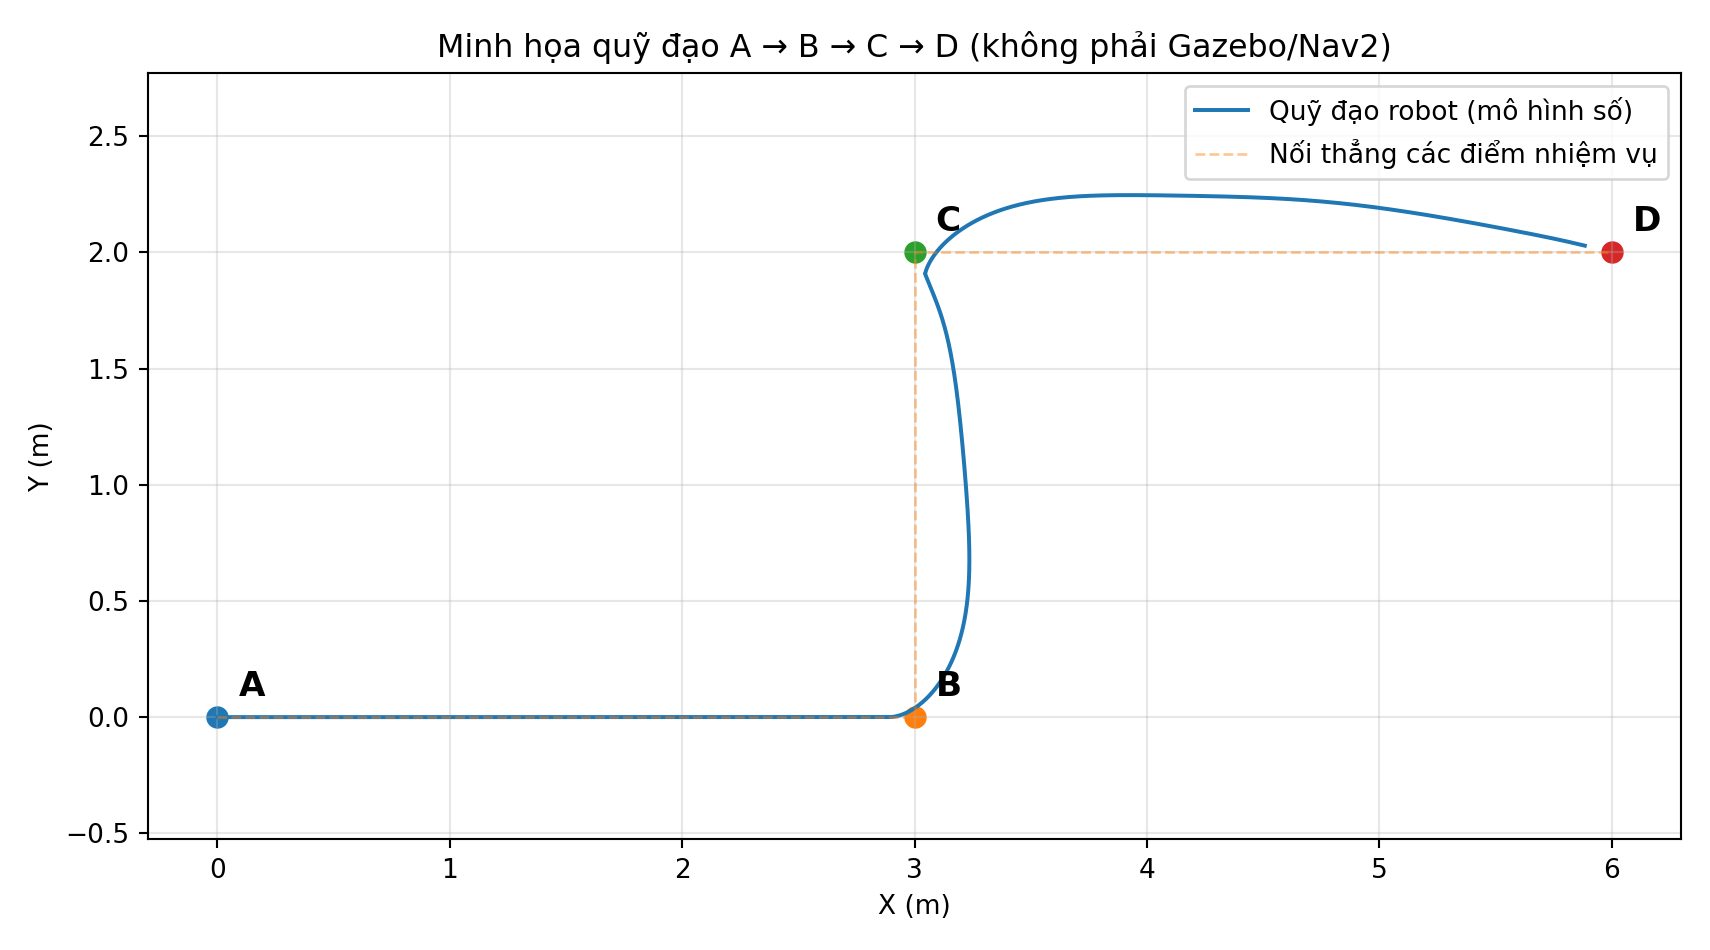
\includegraphics{assets/extended_waypoint_abcd.png}
\caption{Đường đi minh họa đến B, C và D. Các tọa độ không phải bản đồ
kho thật.}
\end{figure}

Tọa độ được chọn để kiểm tra thuật toán trên mặt phẳng, không lấy từ sơ
đồ nhà máy:

\begin{longtable}[]{@{}lrr@{}}
\toprule\noalign{}
Điểm & \(x\) (m) & \(y\) (m) \\
\midrule\noalign{}
\endhead
\bottomrule\noalign{}
\endlastfoot
A & 0 & 0 \\
B & 3 & 0 \\
C & 3 & 2 \\
D & 6 & 2 \\
\end{longtable}

\begin{figure}
\centering
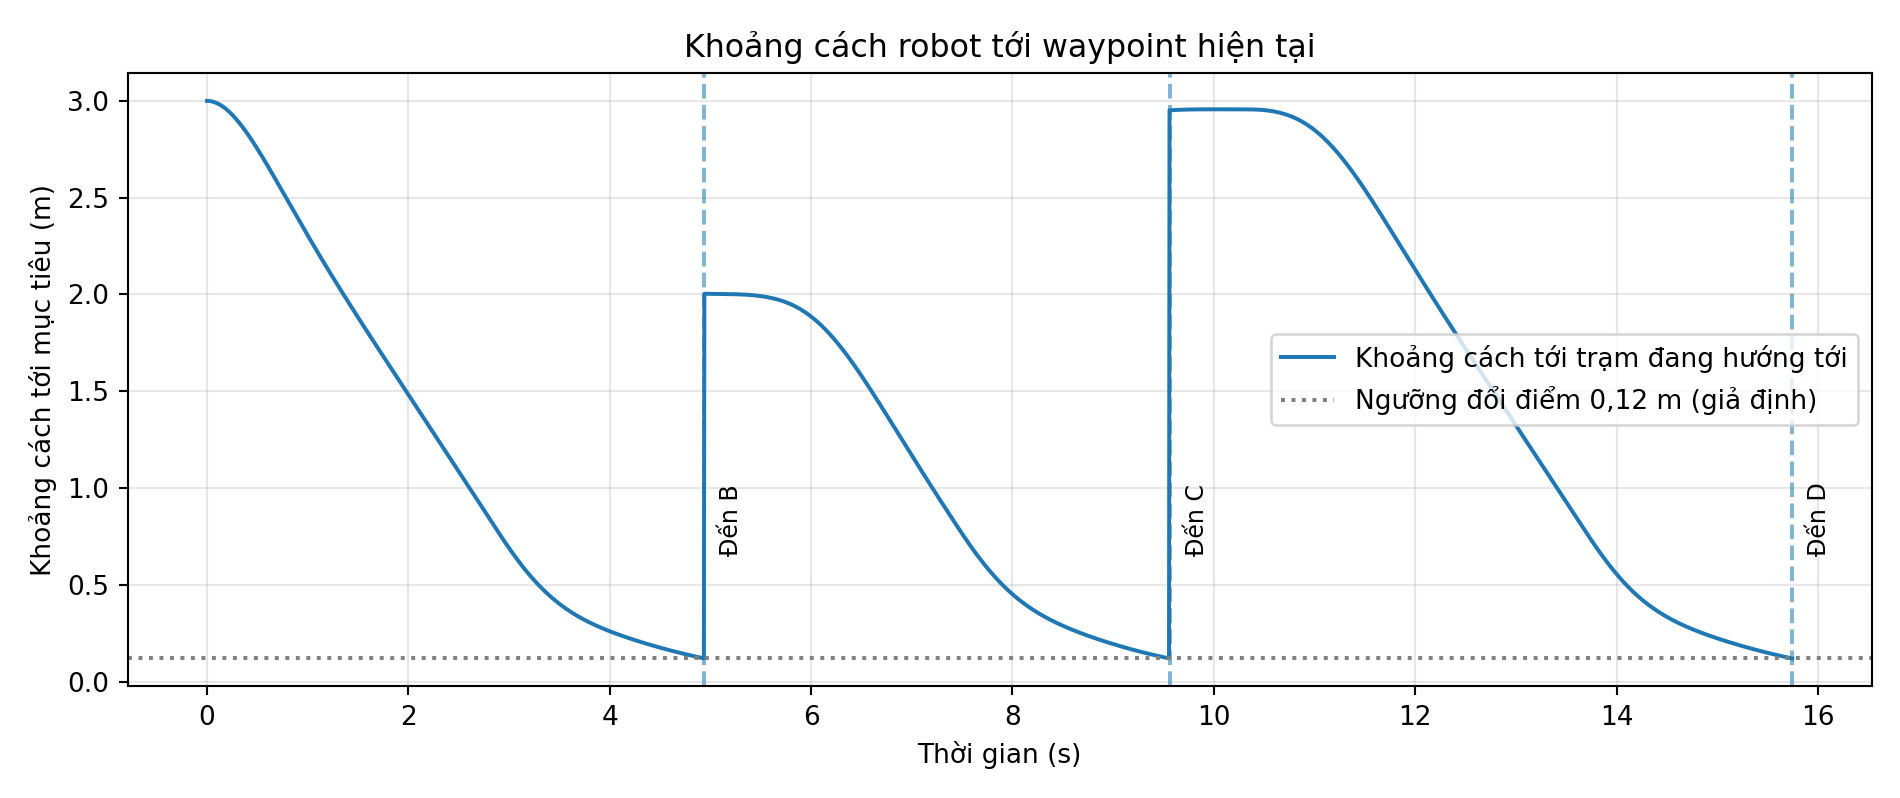
\includegraphics{assets/extended_waypoint_distance.png}
\caption{Khoảng cách tới waypoint đang phục vụ. Đường ngưỡng là 0,12 m.}
\end{figure}

Thời điểm chuyển điểm trong lần chạy Python mẫu: B tại \textbf{4,94 s},
C tại \textbf{9,56 s} và D tại \textbf{15,745 s}. Ngưỡng kích hoạt
chuyển điểm là \(0,12\) m tức 120 mm, \textbf{không đạt và cũng không
dùng để chứng minh tiêu chí dừng nhỏ hơn 30 mm}. Bộ điều khiển waypoint
này không tích hợp SLAM/Nav2, vật cản hay an toàn người đi bộ.

\subsection{6.6. Tình trạng kiểm
chứng}\label{tuxecnh-trux1ea1ng-kiux1ec3m-chux1ee9ng}

\begin{longtable}[]{@{}
  >{\raggedright\arraybackslash}p{(\columnwidth - 2\tabcolsep) * \real{0.5000}}
  >{\raggedright\arraybackslash}p{(\columnwidth - 2\tabcolsep) * \real{0.5000}}@{}}
\toprule\noalign{}
\begin{minipage}[b]{\linewidth}\raggedright
Hạng mục
\end{minipage} & \begin{minipage}[b]{\linewidth}\raggedright
Kết luận ở phiên bản tài liệu này
\end{minipage} \\
\midrule\noalign{}
\endhead
\bottomrule\noalign{}
\endlastfoot
Phương trình động học và quy đổi hai bánh & Đã kiểm tra bằng các bài thử
số Python \\
Chương trình Python và dữ liệu CSV & Đã chạy, có thể tái tạo lại hình \\
Mô hình MATLAB \texttt{.m} & Đã rà soát tĩnh; chưa kiểm chứng runtime
MATLAB \\
Gazebo / ROS 2 / Nav2 & Chưa chạy kiểm tra trong lần cập nhật này \\
Động cơ 48 V - 250 W, hộp số, pin & Chỉ là phương án sơ bộ, chưa đối
chiếu datasheet/URDF \\
Dừng chính xác dưới 30 mm và an toàn với người & Chưa có bằng chứng
nghiệm thu \\
\end{longtable}

\section{7. Bộ mã MATLAB và quy trình tái
lập}\label{bux1ed9-muxe3-matlab-vuxe0-quy-truxecnh-tuxe1i-lux1eadp}

\subsection{7.1. Cấu trúc và chức
năng}\label{cux1ea5u-truxfac-vuxe0-chux1ee9c-nux103ng}

Tất cả mã MATLAB được đặt dưới
\texttt{research/diff\_drive\_pid/matlab/}. Bộ mã bao gồm \textbf{16
file \texttt{.m}}, có chức năng mô hình hóa động học thuận/nghịch, mô
phỏng phương trình quán tính ghép hai bánh, chạy các bộ P/PI/PID và lưu
ảnh, dữ liệu thô. Không yêu cầu Simulink hoặc Control System Toolbox
trong luồng \texttt{run\_all}. Nhóm có thể mở rộng lên Simulink sau khi
đồng bộ với URDF và hệ điều khiển thật.

\begin{longtable}[]{@{}
  >{\raggedright\arraybackslash}p{(\columnwidth - 4\tabcolsep) * \real{0.3333}}
  >{\raggedright\arraybackslash}p{(\columnwidth - 4\tabcolsep) * \real{0.3333}}
  >{\raggedright\arraybackslash}p{(\columnwidth - 4\tabcolsep) * \real{0.3333}}@{}}
\toprule\noalign{}
\begin{minipage}[b]{\linewidth}\raggedright
Nhóm mã
\end{minipage} & \begin{minipage}[b]{\linewidth}\raggedright
File MATLAB chính
\end{minipage} & \begin{minipage}[b]{\linewidth}\raggedright
Vai trò
\end{minipage} \\
\midrule\noalign{}
\endhead
\bottomrule\noalign{}
\endlastfoot
Hằng số và động học & \texttt{amr\_params.m},
\texttt{diffdrive\_forward.m}, \texttt{diffdrive\_inverse.m} & Thông số,
động học bánh và thân \\
Vòng điều khiển & \texttt{wheel\_pi\_step.m},
\texttt{wheel\_pid\_step.m} & PI có anti-windup, PID có lọc D \\
Kịch bản & \texttt{simulate\_straight\_pi.m},
\texttt{simulate\_turning.m}, \texttt{simulate\_p\_vs\_pi.m} & Đi thẳng,
rẽ và nhiễu tải \\
Quỹ đạo \& PID & \texttt{simulate\_waypoints.m} & A--B--C--D \\
So sánh PI/PID & Mã mô phỏng PI/PID & Chạy với tham số minh họa \\
Xuất và kiểm tra & \texttt{amr\_plot\_all.m},
\texttt{amr\_write\_csv.m}, \texttt{amr\_save\_png.m},
\texttt{validate\_amr.m} & Hình, CSV, smoke tests \\
Chạy toàn bộ & \texttt{run\_all.m}, \texttt{plot\_from\_python\_csv.m} &
Điều phối và đọc dữ liệu đối chiếu \\
\end{longtable}

File dùng trong dòng so sánh PI/PID là
\texttt{simulate\_pi\_pid\_comparison.m}.

\subsection{7.2. Chạy toàn bộ trên
MATLAB}\label{chux1ea1y-touxe0n-bux1ed9-truxean-matlab}

Mở MATLAB, di chuyển đến thư mục
\texttt{research/diff\_drive\_pid/matlab} trong bản clone GitHub của
nhóm:

\begin{Shaded}
\begin{Highlighting}[]
\VariableTok{cd}\NormalTok{(}\SpecialStringTok{\textquotesingle{}C:\textbackslash{}Users\textbackslash{}nghoa\textbackslash{}Desktop\textbackslash{}Industrial\_AMR\_Robot\textbackslash{}research\textbackslash{}diff\_drive\_pid\textbackslash{}matlab\textquotesingle{}}\NormalTok{)}
\VariableTok{run\_all}
\end{Highlighting}
\end{Shaded}

Sau khi chạy thành công, chương trình dự kiến tạo \textbf{14 ảnh
\texttt{matlab\_*.png}} tại \texttt{docs/assets/} và \textbf{7 CSV
\texttt{matlab\_*.csv}} tại \texttt{examples/data/}. Các ảnh này được
xuất từ MATLAB trên máy người thực hiện, \textbf{không nằm sẵn trong báo
cáo này} vì máy biên soạn không có MATLAB. Không đổi tên ảnh
\texttt{extended\_*.png} thành \texttt{matlab\_*.png} vì làm vậy sẽ sai
nguồn chứng cứ.

Nếu \texttt{run\_all} báo lỗi, ghi log MATLAB, phiên bản MATLAB và tệp
\texttt{.m} gây lỗi; chỉ đưa ảnh MATLAB vào tài liệu sau khi kiểm tra
kết quả trực tiếp. MATLAB \texttt{validate\_amr.m} chỉ là smoke test
tính nhất quán số, không phải thử nghiệm nghiệm thu khách hàng.

\subsection{7.3. Chạy Python đối chiếu và cập nhật
PDF}\label{chux1ea1y-python-ux111ux1ed1i-chiux1ebfu-vuxe0-cux1eadp-nhux1eadt-pdf}

Tại thư mục \texttt{research/diff\_drive\_pid/}:

\begin{Shaded}
\begin{Highlighting}[]
\NormalTok{python }\OperatorTok{{-}}\NormalTok{m pip install numpy matplotlib}
\NormalTok{python examples}\OperatorTok{/}\NormalTok{simulate\_diff\_drive\_pi}\OperatorTok{.}\FunctionTok{py}
\NormalTok{python examples}\OperatorTok{/}\NormalTok{simulate\_extended\_plots}\OperatorTok{.}\FunctionTok{py}
\NormalTok{python examples}\OperatorTok{/}\NormalTok{simulate\_pi\_pid\_comparison}\OperatorTok{.}\FunctionTok{py}
\end{Highlighting}
\end{Shaded}

Lệnh đầu tạo profile đi thẳng, lệnh hai tạo chín biểu đồ mở rộng và các
CSV, lệnh ba tạo so sánh PI/PID bổ sung. Mỗi ảnh đều có một script tái
lập và được lưu trong \texttt{docs/assets/}. Chương trình không sử dụng
mô hình kho Gazebo hoặc dữ liệu từ robot thật.

\subsection{7.4. Đối chiếu với robot thật và bài thử tiếp
theo}\label{ux111ux1ed1i-chiux1ebfu-vux1edbi-robot-thux1eadt-vuxe0-buxe0i-thux1eed-tiux1ebfp-theo}

Trước khi đưa PID lên controller của robot, cần kiểm tra cấu hình URDF
hiện hành (\texttt{wheel\_radius}, \texttt{wheel\_separation}, khối
lượng, mô-men quán tính), tỷ số truyền và driver, chu kỳ điều khiển
thực, dấu encoder và phương án chống mất lệnh. Nếu driver đã tự điều tốc
bằng FOC/PID, không tạo hai vòng tốc độ xung đột. Để nghiệm thu, cần log
ROS 2/Gazebo hoặc robot thật với nguồn dữ liệu và thời gian cụ thể; đặc
biệt phải có bài test độ chính xác docking, khả năng phanh và khả năng
vận hành dưới tải.

\section{8. Kết luận}\label{kux1ebft-luux1eadn}

Báo cáo đã tổng hợp cơ sở động học, động lực học và PID của robot AMR
truyền động vi sai, có mô hình quán tính ghép hai bánh, tính chọn sơ bộ
lực kéo--mô-men, phương pháp mô phỏng và phân tích hình ảnh. Bộ mã
MATLAB 16 tệp, bộ mã Python và dữ liệu CSV được sắp xếp chung trong cùng
thư mục để nhóm sử dụng khi viết báo cáo và làm slide.

Kết quả chạy Python cho thấy mô hình số có thể tái hiện các chuyển động
đi thẳng, vào cua, quay tại chỗ, phản ứng P/PI/PID khi tải thay đổi và
nhiệm vụ waypoint A--B--C--D minh họa. Các số liệu này \textbf{không xác
nhận} hiệu năng, an toàn hoặc độ chính xác của AMR do nhóm chế tạo. Giai
đoạn tiếp theo cần chạy \texttt{run\_all.m} trên MATLAB của thành viên,
so khớp với URDF và kiểm chứng Gazebo/ROS 2 bằng ảnh, log và kịch bản
thử nghiệm thực tế.

\section{Tài liệu tham khảo}\label{tuxe0i-liux1ec7u-tham-khux1ea3o}

\begin{enumerate}
\def\labelenumi{\arabic{enumi}.}
\tightlist
\item
  ROS 2 Control:
  \href{https://control.ros.org/jazzy/doc/ros2_controllers/diff_drive_controller/doc/userdoc.html}{diff\_drive\_controller
  (Jazzy)}.
\item
  ROS 2 Documentation:
  \href{https://docs.ros.org/en/jazzy/Concepts/Intermediate/About-Tf2.html}{About
  tf2}.
\item
  Gazebo: \href{https://gazebosim.org/docs/harmonic/}{Gazebo Harmonic
  documentation}.
\item
  Repository nhóm:
  \href{https://github.com/HoangAnh301194/Industrial_AMR_Robot}{Industrial\_AMR\_Robot}
  (thông số động lực học phải được kiểm tra với cấu hình phiên bản hiện
  hành).
\end{enumerate}

\end{document}
